\documentclass[fleqn,10pt]{wlscirep}

\usepackage[utf8]{inputenc}
\usepackage[T1]{fontenc}
\usepackage{graphicx}
\usepackage{tabularx}
\usepackage{array}
\usepackage{amsmath}
\usepackage[none]{hyphenat}

\graphicspath{{../figures/}{../}}
\makeatletter
\def\input@path{{../}}
\makeatother
\setlength{\emergencystretch}{5em}

\newenvironment{paperwidefigure}{\begin{figure}[htbp]}{\end{figure}}
\newenvironment{paperinlinefigure}{\begin{figure}[htbp]}{\end{figure}}
\newenvironment{paperwidetable}{\begin{table}[htbp]}{\end{table}}

% Shared sections use natbib-style citation commands; Scientific Reports uses cite.
\providecommand{\citep}[1]{\cite{#1}}

\title{Sparse Biomarker Discovery from Low-Montage Resting-State EEG for tDCS Treatment Response in Adults with Treatment-Resistant Depression}

\author[1,*]{Abin Daniel Zorto}
\author[2]{Jijomon C. Moncy}
\author[1]{Mhd Saeed Sharif}
\author[2]{Cynthia H.Y. Fu}

\affil[1]{Intelligent Technologies Research Group, University of East London, London, E16 2RD, UK}
\affil[2]{School of Psychology, University of East London, London, E16 2RD, UK}
\affil[*]{u2091940@uel.ac.uk}

\keywords{resting-state EEG, transcranial direct current stimulation, major depressive disorder, treatment-resistant depression, biomarker discovery, low-montage EEG}

\begin{abstract}
We evaluated whether sparse feature selection from 4-channel resting-state EEG could identify remission predictors in a home-based tDCS trial for major depression. Across 150 configurations of a hybrid CNN-LSTM and linear SVM, we varied window length (2--10~s) and feature budget (1--70) under leave-one-participant-out cross-validation with SMOTE.

The strongest hybrid configuration (6~s windows, one feature per fold) achieved patient-level ROC-AUC~0.816, PR-AUC~0.579, balanced accuracy~0.786, and MCC~0.571 over 21 held-out participants. A permutation test confirmed above-chance discrimination (raw $p=0.008$; 2-family Bonferroni-corrected $p_\text{corr}=0.016$), although significance does not survive correction for the full 150-configuration sweep. The best SVM (8~s, 30 features) reached ROC-AUC~0.510 ($p=0.469$, uncorrected). The hybrid model exhibited extreme sparsity: only 7 unique features appeared across folds, with modest overlap (mean Jaccard~0.190) but perfect effect-direction consistency among recurrent features.

These findings suggest that patient-level discrimination signals are recoverable from highly sparse representations of low-montage EEG. The recurrent features centred on temporal spectral entropy and frontal-temporal difference measures, converging with prior analyses in the same cohort. The results support low-montage resting-state EEG as a basis for pretreatment stratification research, pending independent validation.

\end{abstract}

\begin{document}

\flushbottom
\maketitle
\thispagestyle{empty}

\section*{Introduction}
Major depressive disorder (MDD) remains a leading cause of global disability and is characterized by marked heterogeneity in clinical presentation, neurobiology, and treatment response. Despite the availability of pharmacological and psychotherapeutic interventions, a substantial proportion of patients fail to achieve remission, motivating increasing interest in neuromodulation approaches such as transcranial direct current stimulation (tDCS) \citep{Woodham2021}. While randomized controlled trials and recent large-scale studies support the feasibility and clinical potential of tDCS, including fully remote, home-based delivery, treatment outcomes remain variable at the individual level \citep{woodham2025home,Hampsey2026}.

Home-based delivery has moved from concept to clinical trial: a fully remote phase 2 randomized sham-controlled study demonstrated home-based tDCS in major depressive disorder \citep{woodham2025home}, and qualitative follow-up work found the approach acceptable to participants \citep{Rimmer2024}. These advances make pretreatment stratification a practical clinical problem. A central challenge is pretreatment stratification: identifying which patients are more likely to achieve remission before treatment begins. Electroencephalography (EEG) is a potential modality for this purpose due to its portability, low cost, and high temporal resolution.

The literature on EEG biomarkers in major depressive disorder is encouraging though methodologically uneven. Reviews and biomarker overviews have repeatedly highlighted spectral, asymmetry, vigilance, entropy, and complexity signatures as potentially informative marker families \citep{olbrich2013_eeg,olbrich2015_personalized,leuchter2010_biomarkers}. Related discussions of neuroimaging and EEG biomarkers have emphasized the clinical opportunity, but also the need for more robust treatment-response models and better translational discipline \citep{Fu2013,Fu2019,Widge2019}. More recent meta-analytic work on EEG-based treatment prediction reaches a similar conclusion: useful signal is present, but translation depends on stronger methodology and standardization \citep{simmatis2023_technical,watts2022predicting,cohen2023electroencephalography}. Machine learning studies have extended this literature into antidepressant, placebo, and neuromodulation response prediction, while also exposing recurrent concerns about external generalization, feature stability, leakage-safe selection, and interpretability \citep{AlKaysi2017,jaworska2019_leveraging,oakley2022_eeg}. Related nonlinear and entropy-oriented studies point to the same caution about dimensionality and signal instability \citep{shalbaf2018_nonlinear,ebrahimzadeh2021_predicting,zhdanov_svm_prediction}. Entropy-focused EEG work has reinforced the relevance of complexity measures \citep{Puthankattil2012,Ghiasi2021,Zhao2022}. Leakage-specific and data-centric critiques make the underlying design problem explicit \citep{Shim2021,Shen2025}.

That tension is especially sharp in relatively small neuromodulation studies. Rich models can improve representation learning, but relatively small cohorts also increase the risk of unstable feature selection, inflated performance estimates, and overly confident biomarker claims. Nested evaluation and within-fold processing are therefore central design issues rather than implementation details in this literature \citep{Widge2019,Shim2021}. Clinically deployable EEG biomarkers also need interpretability and low-density feasibility, and recent data-centric frameworks have started to move in that direction \citep{Shen2025}. Emerging response-prediction studies in depression and related neuromodulation settings show substantial promise \citep{funk2008_prefrontal,bailey2023_concurrent,murphy2023_neural}. Related reviews and pilot studies also make the methodological fragility clear \citep{guo2024_restingstate,tsai2023_review,Dagnino2023}. More recent response-oriented studies continue that pattern \citep{sheen2024_response,zeidabadi2025_prediction,reissmann2026_thetacordance}. A recent systematic review of EEG connectivity changes in depression treatment reaches a similar conclusion \citep{ulrich2025_alterations}.

Within the same home-based 4-channel MDD program analysed here, power spectral density (PSD)-based and PLV-based analyses have observed that the baseline EEG carries treatment-response information across multiple signal representations \citep{Moncy2024,Xiao2025PMIP}. PSD-based deep learning approaches identified temporoparietal spectral features, notably TP10 theta-alpha power, as informative for treatment outcome prediction \citep{Moncy2024}, while connectivity-based analyses highlighted frontal-temporal and temporoparietal network patterns \citep{Xiao2025PMIP}. Together, these findings suggest that response-related signal is present and reproducible across feature families, but remains poorly characterized in terms of interpretability, stability, and minimal feature representation.

The present study builds directly on this context and uses the same baseline EEG cohort as our prior PSD- and connectivity-based analyses \citep{Moncy2024,Xiao2025PMIP}, but addresses a distinct question. Rather than optimising predictive performance within a predefined feature family, we test whether a strictly leakage-controlled, foldwise sparse feature-selection pipeline can identify a small, recurrent, and interpretable biomarker set under participant-level validation. We compared two classifiers over the same feature-selection sweep to test whether low-montage resting-state EEG could recover a small recurring set of biomarkers associated with tDCS remission in adults with MDD. The analysis prioritized parsimony, biomarker interpretability, and leakage-resistant participant-level validation. Our working hypothesis was that useful patient-level discrimination could be achieved with a small per-fold feature budget and that the most recurrent features would show stronger effect-direction consistency than hard-set overlap. This approach reframes biomarker discovery from a high-dimensional modelling problem toward a minimal, interpretable signal identification problem.


\section*{Methods}
\subsection{Dataset and signal representation}

The analysis used pretreatment EEG from 21 adults with treatment-resistant depression enrolled in a fully remote, multisite, double-blind, randomized sham-controlled home-based tDCS trial for major depressive disorder \citep{woodham2025home}. The analyzed cohort contained 7 remission cases and 14 non-remission cases in the patient-level outcome labels, with 18 female participants and a mean age of 37.1 $\pm$ 9.7 years. Table~\ref{tab:cohort-summary} summarizes the cohort, acquisition, and sweep configuration.

\begin{table}[H]
  \centering
  \caption{Cohort, acquisition, and sweep configuration summary. Trial descriptors derive from the parent home-based tDCS study \citep{woodham2025home}; acquisition totals and sweep settings derive from the analyzed EEG exports and current experiment configuration.}
  \label{tab:cohort-summary}
  \small
  \begin{tabular}{>{\raggedright\arraybackslash}p{0.42\linewidth}>{\raggedright\arraybackslash}p{0.50\linewidth}}
\toprule
Characteristic & Value \\
\midrule
\multicolumn{2}{l}{\textbf{Parent trial and cohort descriptors}} \\
\addlinespace[0.2em]
Parent trial & Fully remote, multisite, sham-controlled home-based tDCS trial for MDD \citep{woodham2025home} \\
Participants & 21 \\
Outcome groups & 7 remission, 14 non-remission \\
Sex (female/male) & 18/3 \\
Age (years, mean $\pm$ SD) & 37.1 $\pm$ 9.7 \\
\midrule
\multicolumn{2}{l}{\textbf{EEG acquisition and export descriptors}} \\
\addlinespace[0.2em]
Rest condition & Eyes-closed resting state \\
EEG montage & 4 channels (AF7, AF8, TP9, TP10) \\
Channel coverage & Frontal (AF7, AF8), temporal (TP9, TP10) \\
Sampling rate & 256 Hz \\
Recording structure & 10 min total; single file or two 5 min files \\
Available export segment length & 10 s (2,560 samples/channel) \\
Total exported windows & 1,203 \\
Remission windows & 393 (32.7\%) \\
Non-remission windows & 810 (67.3\%) \\
Class ratio & 2.06:1 (non-remission:remission) \\
\midrule
\multicolumn{2}{l}{\textbf{Current sweep methodology settings}} \\
\addlinespace[0.2em]
Sweep window sizes & 2, 4, 6, 8, 10 s \\
Inner-k sweep & 1, 5, 10, 15, 20, 25, 30, 35, 40, 45, 50, 55, 60, 65, 70 \\
Feature selector & SelectKBest ($f$-classif) \\
Training adjustments & LOPO-group equalization + SMOTE \\
Validation & Leave-one-participant-out \\
Evaluation level & Patient-level aggregation \\
\bottomrule
\end{tabular}

\end{table}

Baseline recordings were collected during eyes-closed rest with a 4-channel montage (\texttt{AF7}, \texttt{AF8}, \texttt{TP9}, \texttt{TP10}) sampled at 256 Hz. The available study exports comprised 10 s segments with 2,560 samples per channel, and the underlying recording sessions were stored either as a single 10 min file or as two 5 min files depending on participant. Across the cohort, the export set contained 1,203 windows, including 393 remission-labeled and 810 non-remission-labeled windows. This acquisition setup uses a limited frontal-temporal montage with clear portable-deployment relevance \citep{Casson2010,stoyell2021high}. The montage also constrained the downstream feature space toward frontal, temporal, cross-hemispheric, and frontal-temporal interaction measures.

For the present sweep, the processing configuration applied participant-level per-channel demeaning before upsampling, followed by a fourth-order Butterworth low-pass filter at 60 Hz, a downsampling step back to 256 Hz, and zero-overlap window slicing. The sweep then compared non-overlapping analysis windows of 2, 4, 6, 8, and 10 s, so the model inputs included both the native 10 s exports and shorter subdivisions derived from the same recordings. These choices materially affect downstream EEG feature distributions, especially in low-density or portable pipelines \citep{Siuly2017,Miranda2019,Mahato2020,babiloni2012_guidelines,simmatis2023_technical}. The feature extractor enabled spectral, temporal, entropy, complexity, connectivity, coherence, asymmetry, and cross-hemispheric descriptors, including frontal/temporal asymmetry, cross-regional ratios, and inter-channel coupling measures. This broad handcrafted feature pool was intended to preserve interpretability while allowing sparse downstream selection.

\subsection{Sweep design and validation}

The experiment runner launched two model families over the same feature-selection sweep: an advanced hybrid 1D CNN-LSTM and a linear SVM. All runs used sequential window ordering, SelectKBest with ANOVA $F$ statistics (\texttt{select\_k\_best\_f\_classif}), a fixed consensus feature budget of \texttt{outer-k=10}, leave-one-participant-out outer evaluation, leave-one-participant-out training-group equalization, and SMOTE within training folds. The sweep varied the per-fold feature-selection budget (\texttt{inner-k}) across 15 values from 1 to 70 and repeated the search across 5 window sizes, yielding 150 successful runs in total (75 per model).

This design matters for interpretation. The outer evaluation remained subject independent throughout, so no participant contributed both training and test windows to the same outer fold. The \texttt{inner-k} parameter controlled how many features were selected inside each outer training fold, whereas \texttt{outer-k} controlled only the final consensus feature budget after cross-validation. The feature-selection stability panels in the manuscript describe shared pipeline behavior because both classifiers consumed the same selected features for matched sweep settings.

\subsection{Models}

The SVM baseline used a linear kernel with class-balanced weighting and probability output enabled. The hybrid model used a substantially richer architecture defined in the project model configuration: stacked convolutional blocks, bidirectional LSTM layers, multi-head attention with positional encoding, feature-pyramid fusion, and GELU-activated dense layers with dropout and batch normalization. The manuscript treats this architecture as a test case for whether a more expressive learner can exploit a very small selected feature set more effectively than a linear baseline.

\subsection{Outcome metrics and biomarker summaries}

The primary endpoint was patient-level ROC-AUC, computed from participant probabilities aggregated over held-out windows. Secondary patient-level metrics included PR-AUC, balanced accuracy, accuracy, F1, MCC, precision, recall, and specificity. The pipeline also reported bootstrap confidence intervals and a permutation test for the patient-level ROC-AUC summary. All main manuscript claims use patient-level metrics. Window-level scores appear only as intermediate outputs.

To characterize biomarker behavior across outer folds, we used several post hoc summaries: mean pairwise Jaccard overlap, Kuncheva index, unique feature count, top-feature share, class-conditional selection deltas, and effect-direction consistency. These summaries are descriptive. They characterize recurrence and directionality across folds and do not support causal interpretation. Low overlap can coexist with recurring features that retain consistent class-separation direction when selected \citep{olbrich2013_eeg,olbrich2015_personalized,simmatis2023_technical}.


\section*{Results}
\subsection{Sweep-level comparison}

Across the 150 successful runs (75 hybrid, 75 SVM), the hybrid model outperformed the SVM baseline on patient-level discrimination metrics over most of the sweep landscape. The performance advantage was visible when averaging over window sizes (Figure~\ref{fig:sweep-window-roc}) and when averaging over \texttt{inner-k} settings (Figure~\ref{fig:sweep-innerk-roc}). The best individual hybrid run occurred at 6 s windows with \texttt{inner-k=1}, whereas the best SVM run occurred at 8 s windows with \texttt{inner-k=30}.

To assess statistical robustness across the structured sweep, we applied three correction tiers to the permutation p-values. Treating the sweep as two model-family comparisons (the primary independent factor) yields Bonferroni-corrected $p_\text{corr}=0.016$, confirming that the result survives at $\alpha=0.05$. A max-T permutation correction (10,000 iterations with shared label permutations across all 150 configurations, accounting for inter-configuration correlations) yields $p_\text{corr}=0.302$; the null maximum distribution has mean 0.768 and 95th percentile 0.908, placing the observed maximum of 0.816 within the range expected under random label permutations. The full-sweep Bonferroni ($p_\text{corr}=1.00$) is mechanically uninformative given the 150-test multiplier and is reported for completeness. We adopt the structured 2-family correction as the primary corrected p-value because the window-size and inner-k factors represent exploratory levels of a single hypothesis rather than independent comparisons. Across the sweep, 2 of 150 runs (1.3\%) yielded raw $p<0.05$, and 88\% of runs had $p\ge 0.50$, consistent with a null-dominated landscape from which the best hybrid configuration meaningfully separates.

\begin{paperinlinefigure}
  \centering
  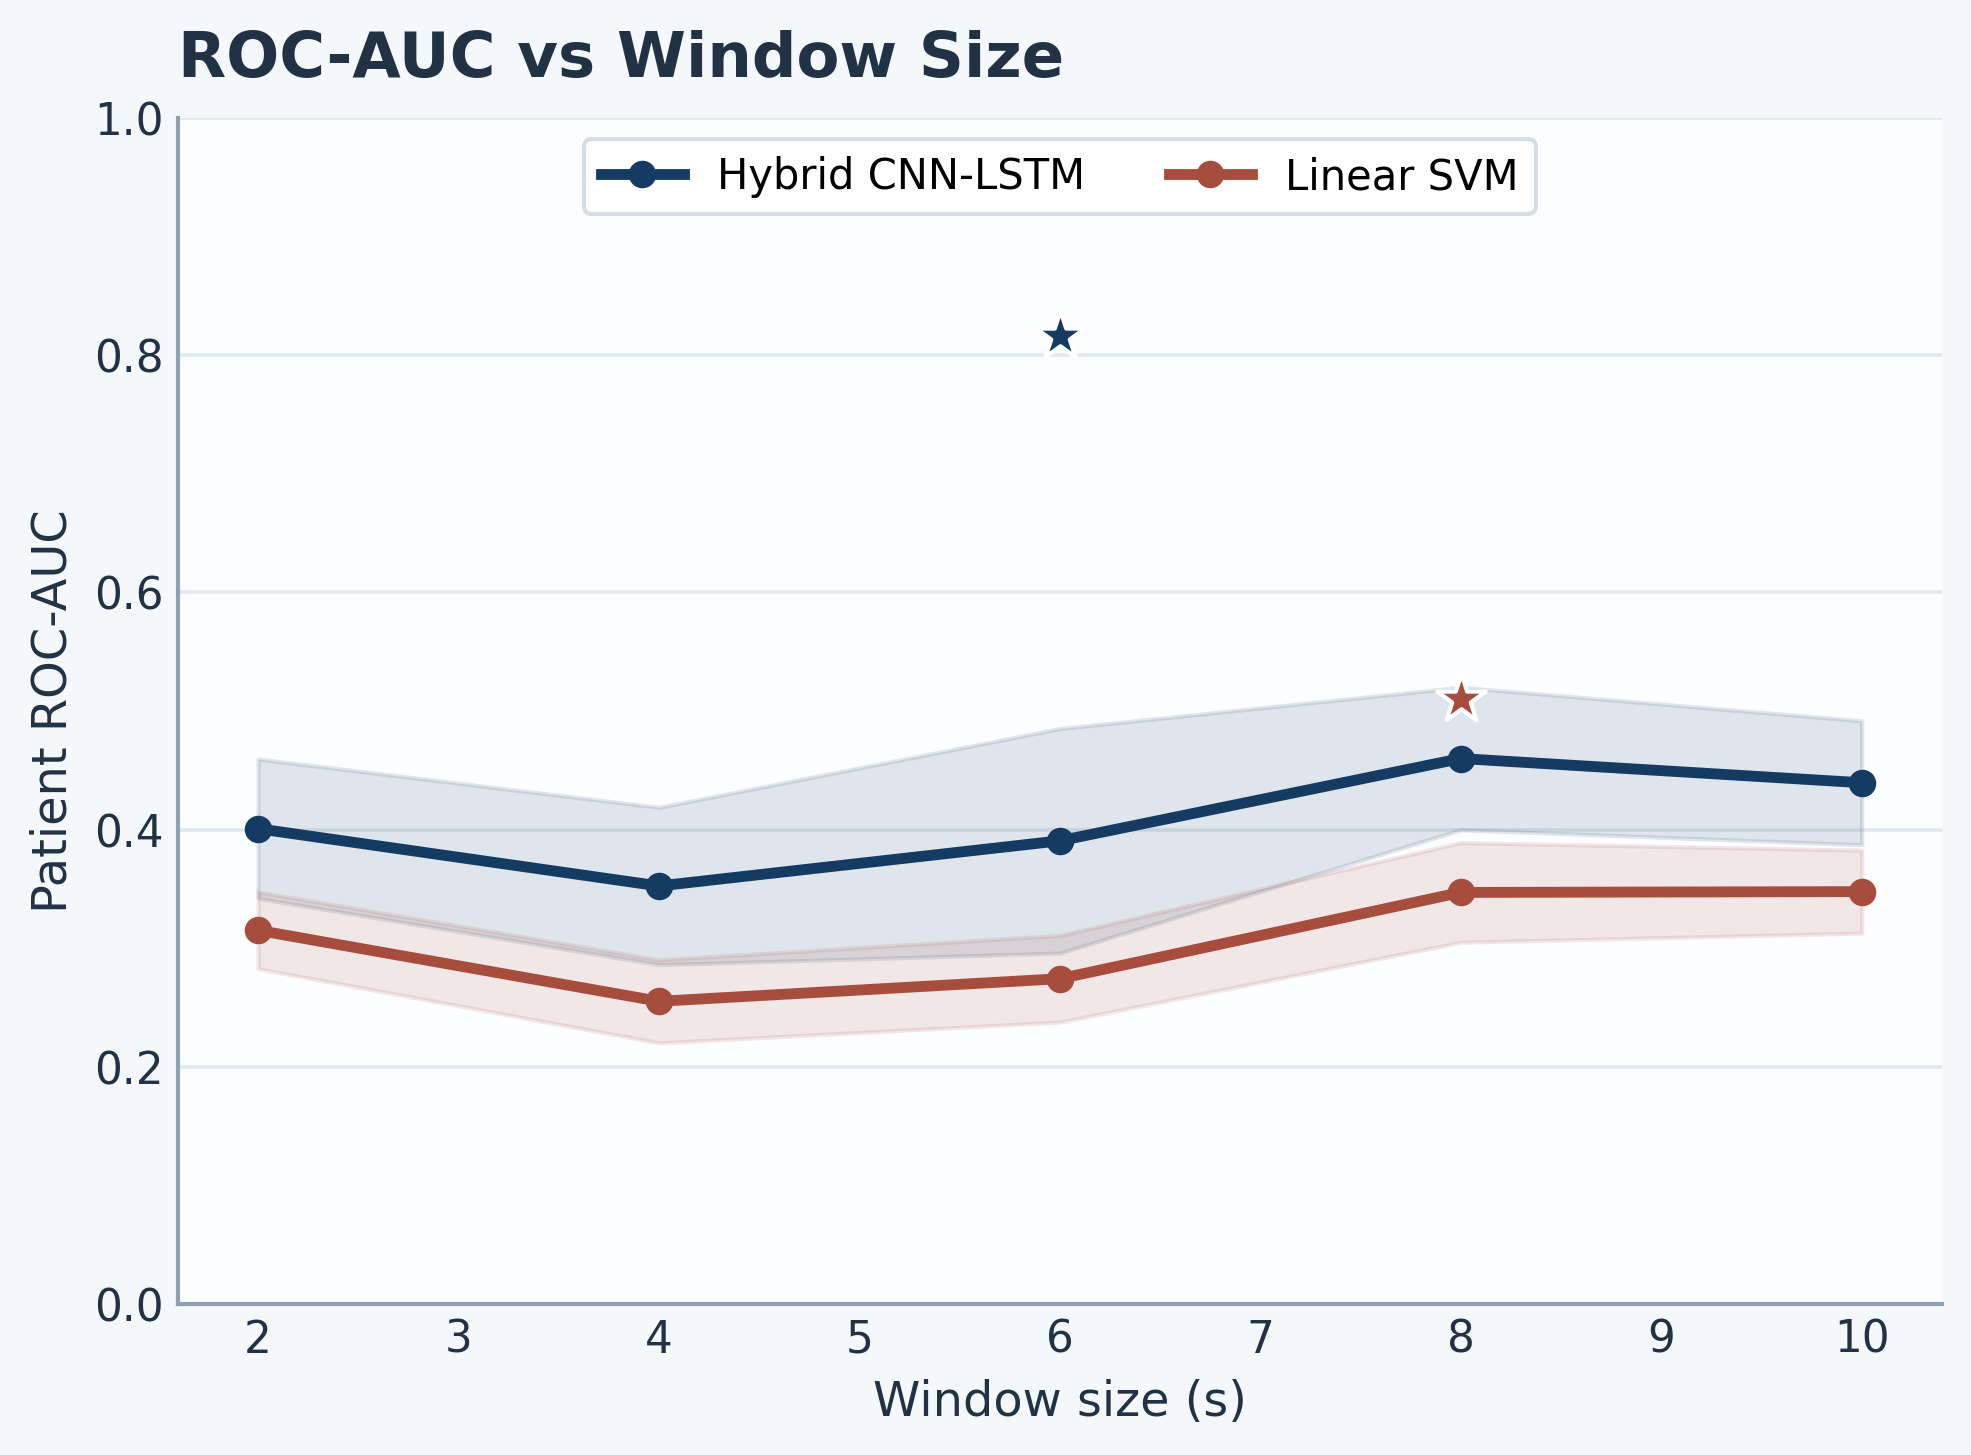
\includegraphics[width=0.94\linewidth]{sweep_window_roc_auc.png}
  \caption{Patient-level ROC-AUC by window size across the sweep. Stars mark the best individual hybrid and SVM runs.}
  \label{fig:sweep-window-roc}
\end{paperinlinefigure}

Figure~\ref{fig:sweep-innerk-roc} shows that the relationship between ROC-AUC and \texttt{inner-k} differed across the two model families in the low-budget region. The hybrid model retained clearly stronger ROC-AUC across the sparsest budgets and achieved the highest individual ROC-AUC in the entire sweep at \texttt{inner-k=1}. The linear SVM did not show the same pattern and reached its best ROC-AUC only at the broader \texttt{inner-k=30} setting. Sparse per-fold selection therefore aligned with peak discrimination only for the more expressive model.

\begin{paperinlinefigure}
  \centering
  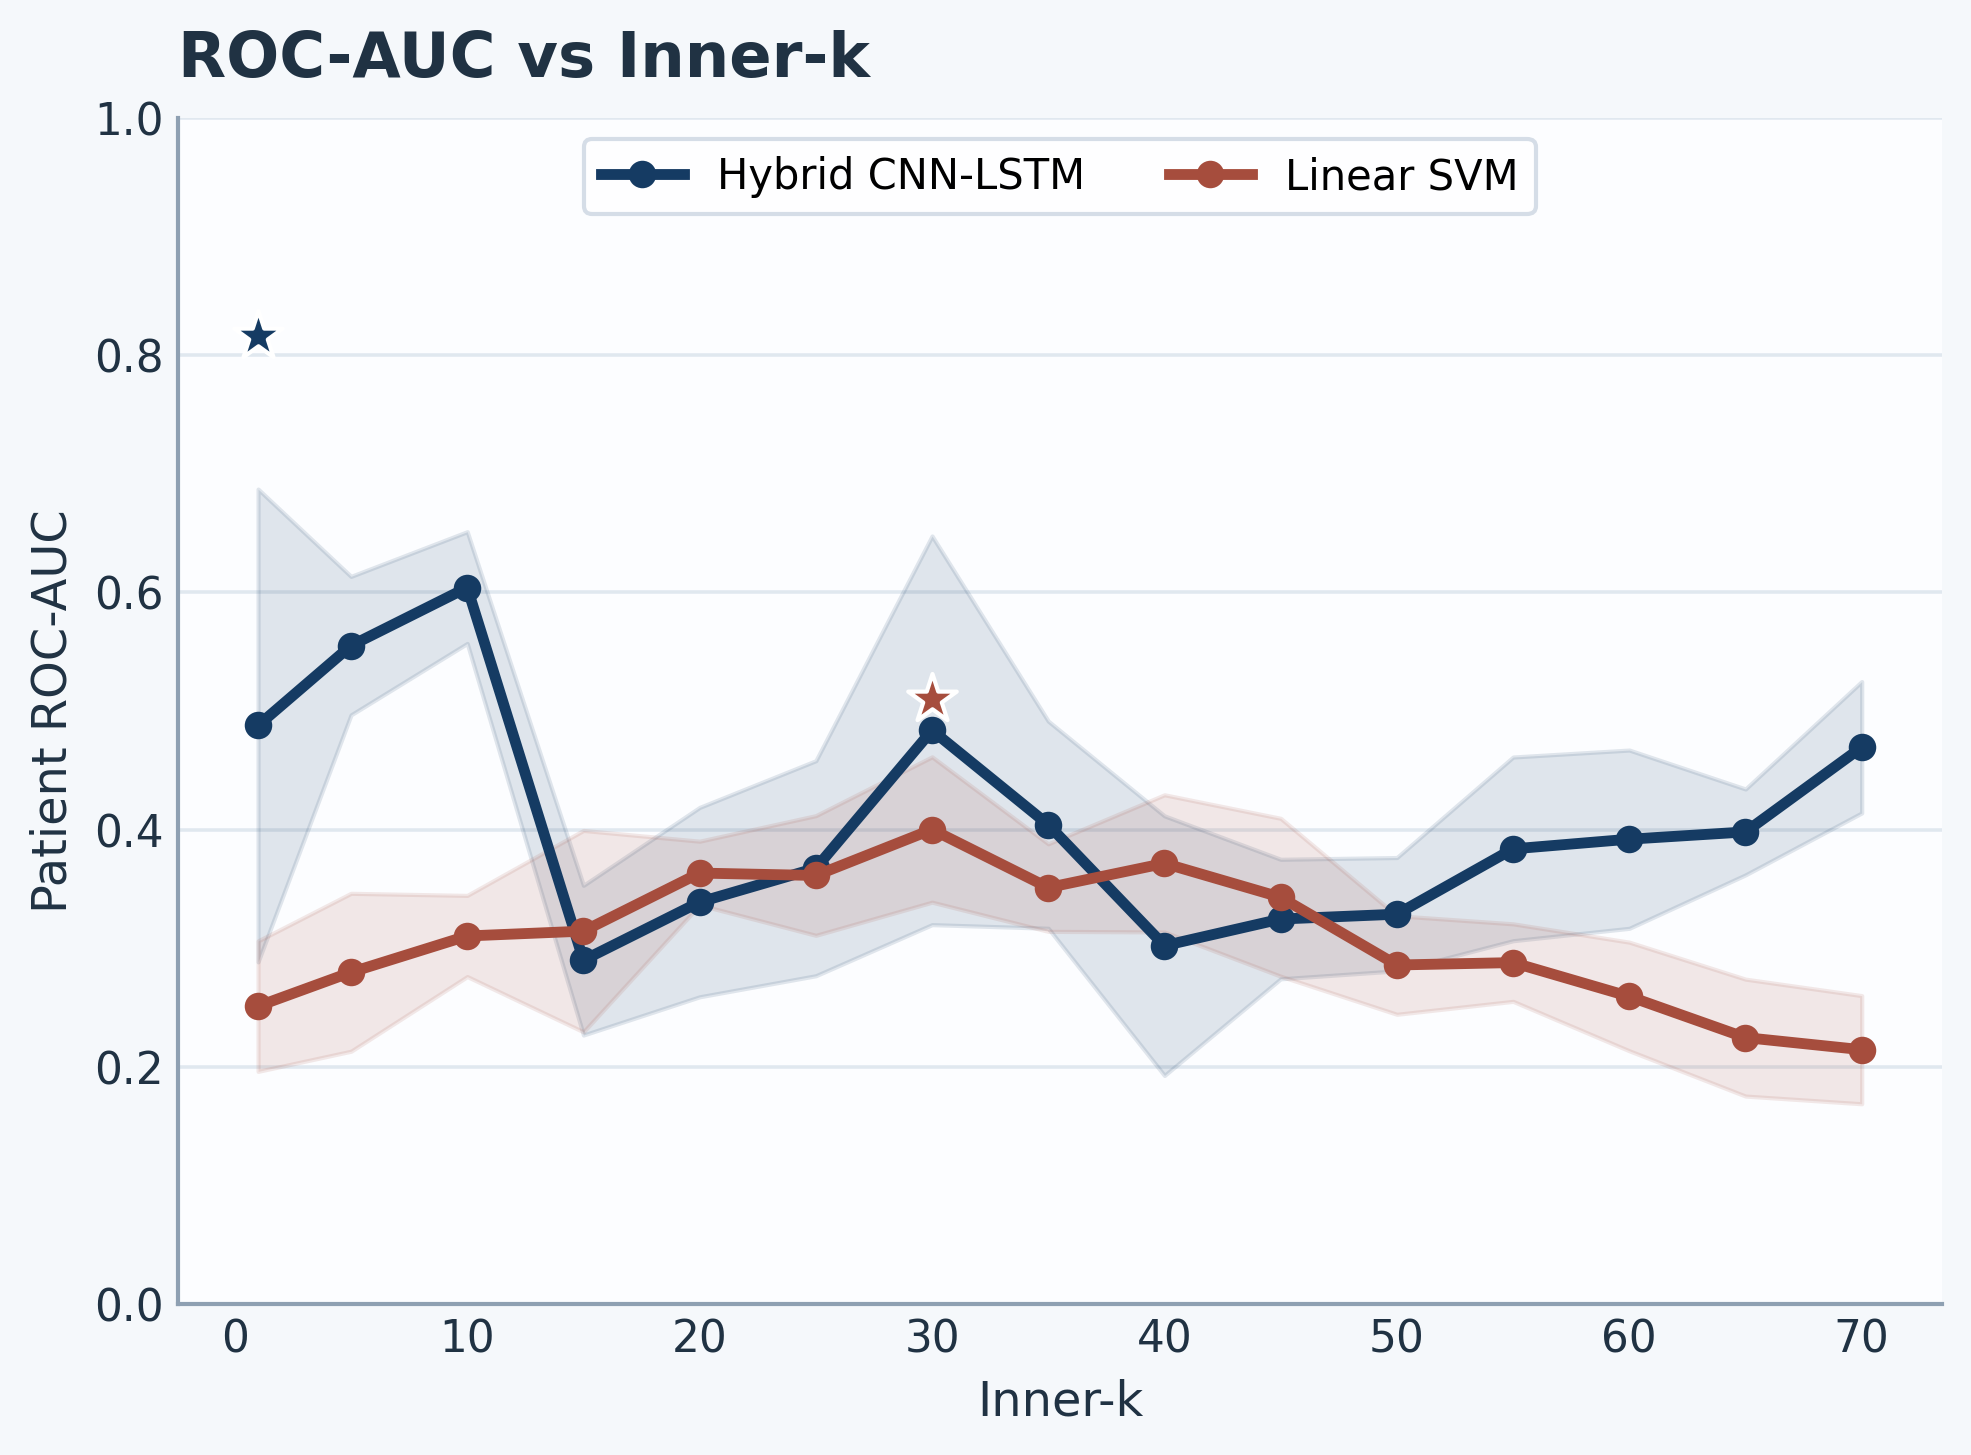
\includegraphics[width=0.94\linewidth]{sweep_inner_k_roc_auc.png}
  \caption{Patient-level ROC-AUC by \texttt{inner-k} across the sweep. The hybrid model retained the strongest discrimination in the sparsest budget region.}
  \label{fig:sweep-innerk-roc}
\end{paperinlinefigure}

Figures~\ref{fig:sweep-jaccard} and \ref{fig:sweep-unique-features} show a second related pattern. Increasing \texttt{inner-k} increased hard-set overlap and the total number of unique selected features. Larger feature budgets did not produce the strongest patient-level discrimination. The sweep concentrated its best hybrid performance at the sparsest end of the per-fold selection range. This pattern suggests that model capacity and per-fold sparsity mattered together rather than independently.

\begin{paperinlinefigure}
  \centering
  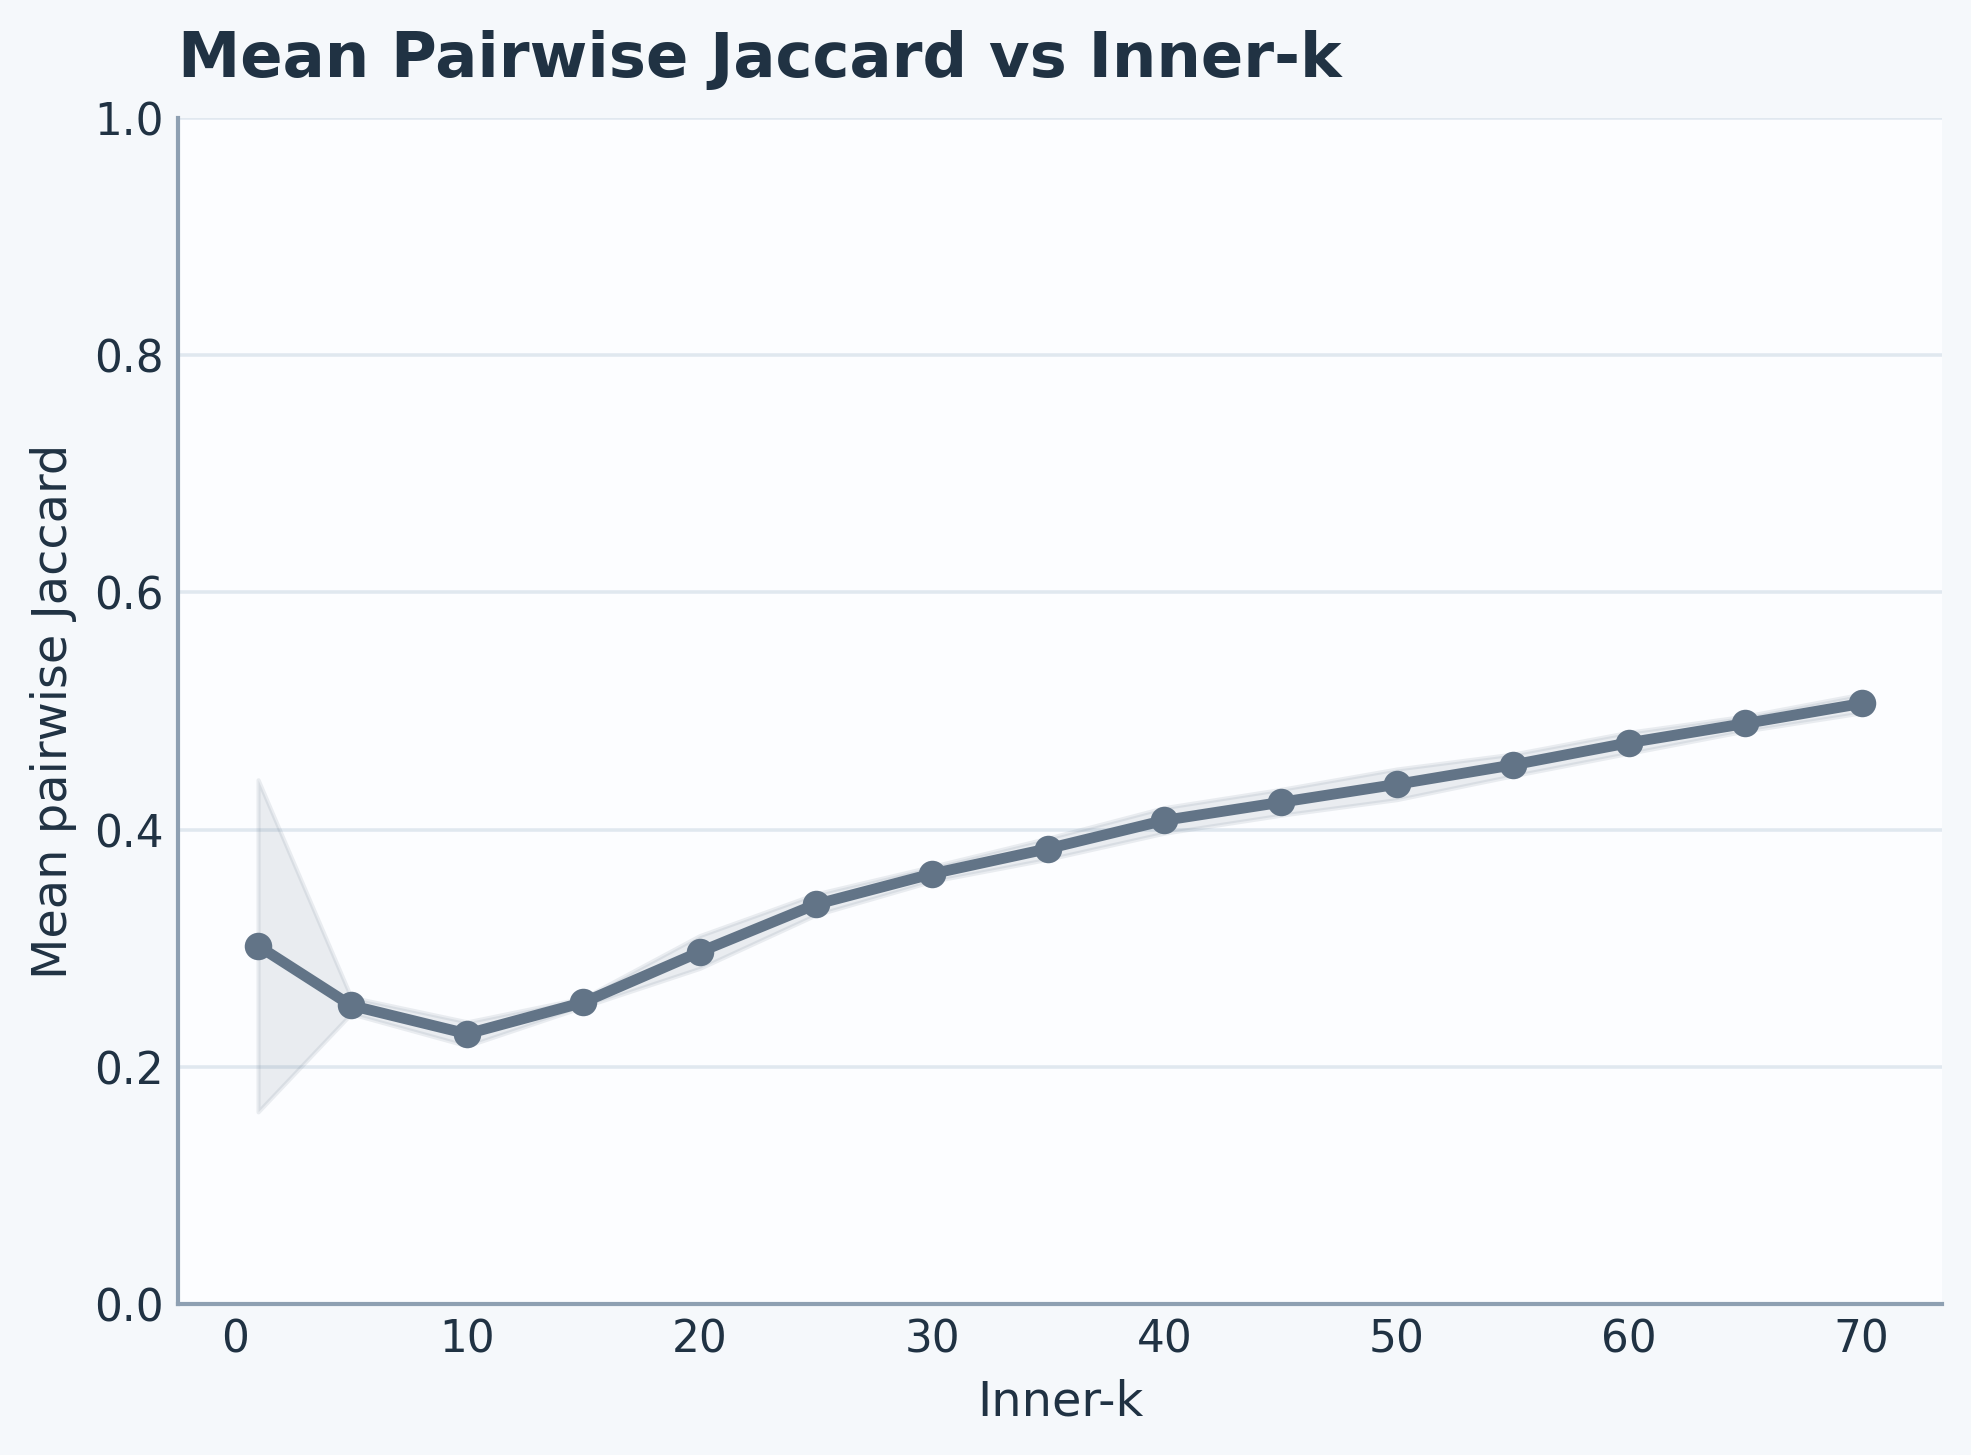
\includegraphics[width=0.94\linewidth]{sweep_jaccard_inner_k.png}
  \caption{Mean pairwise Jaccard overlap by \texttt{inner-k}. Hard-set overlap increased with larger per-fold feature budgets.}
  \label{fig:sweep-jaccard}
\end{paperinlinefigure}

\begin{paperinlinefigure}
  \centering
  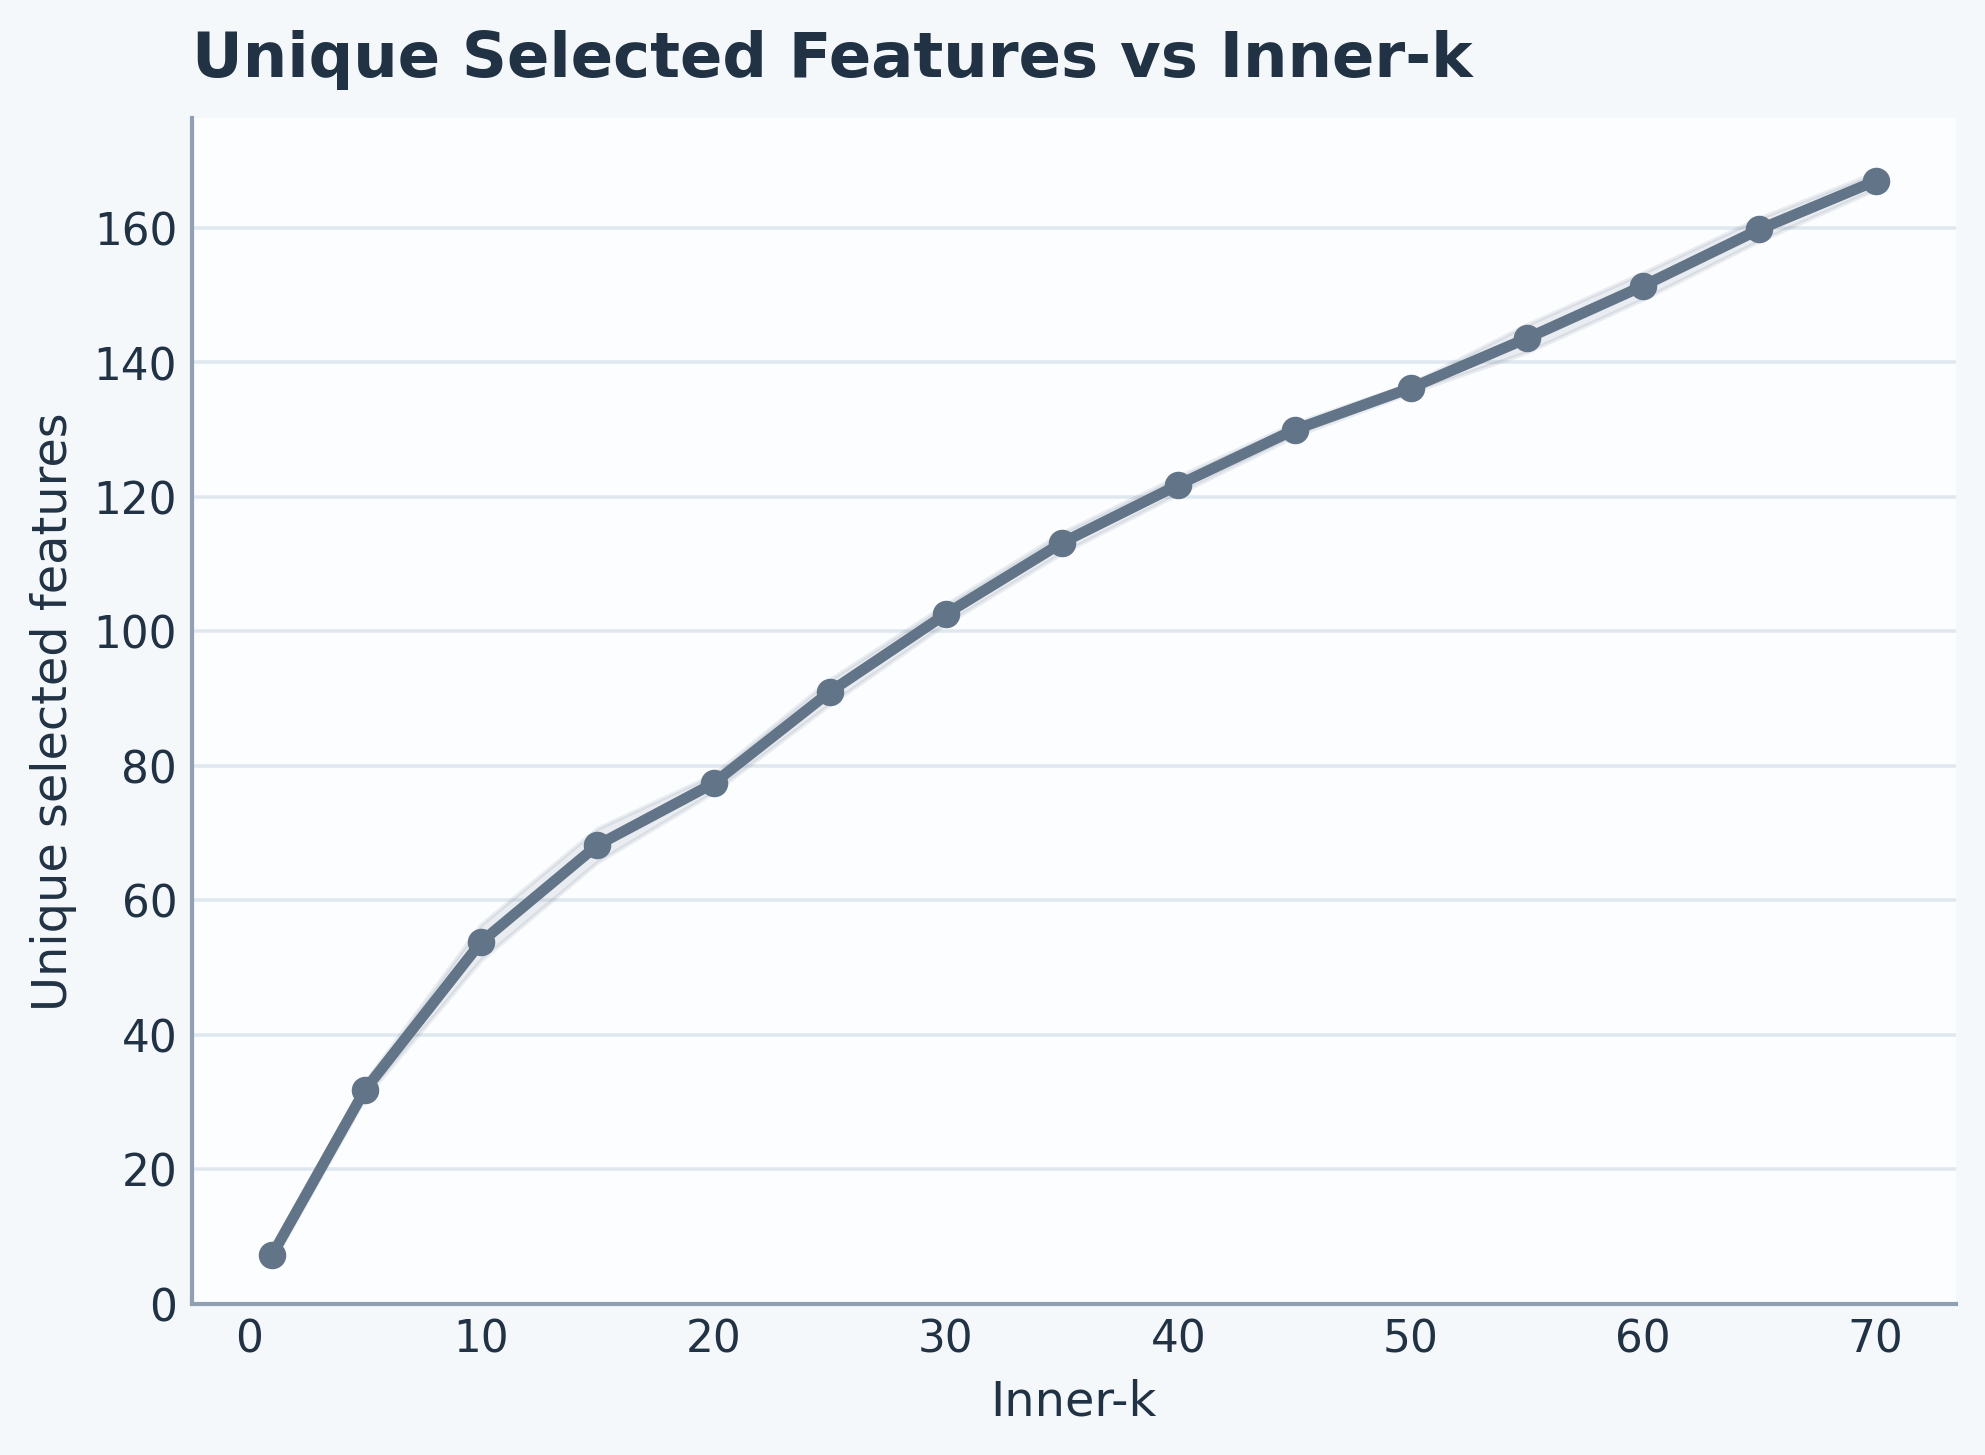
\includegraphics[width=0.94\linewidth]{sweep_unique_features_inner_k.png}
  \caption{Unique selected features by \texttt{inner-k}. Larger per-fold budgets produced markedly larger discovered feature pools.}
  \label{fig:sweep-unique-features}
\end{paperinlinefigure}

\subsection{Best-run patient-level performance}

The best hybrid configuration achieved patient-level ROC-AUC 0.816 [95\% CI: 0.600--0.990], PR-AUC 0.579, balanced accuracy 0.786 [95\% CI: 0.571--0.967], accuracy 0.810 [95\% CI: 0.619--0.952], F1 0.714 [95\% CI: 0.364--0.941], and MCC 0.571 over 21 held-out participants (Figure~\ref{fig:main-roc}; Table~\ref{tab:best-run-comparison}). The permutation test yielded a nominal raw $p=0.008$ based on 500 iterations. Correcting for the structured sweep (2 model families) gives $p_\text{corr}=0.016$, which survives at $\alpha=0.05$; under the more conservative max-T correction across all 150 configurations, $p_\text{corr}=0.302$ (Table~\ref{tab:best-run-comparison} footnote). Bootstrap confidence intervals are wide, reflecting the small sample size of 21 participants. The PR-AUC of 0.579 indicates that the model retained useful precision-recall behavior in this cohort.

\begin{paperinlinefigure}
  \centering
  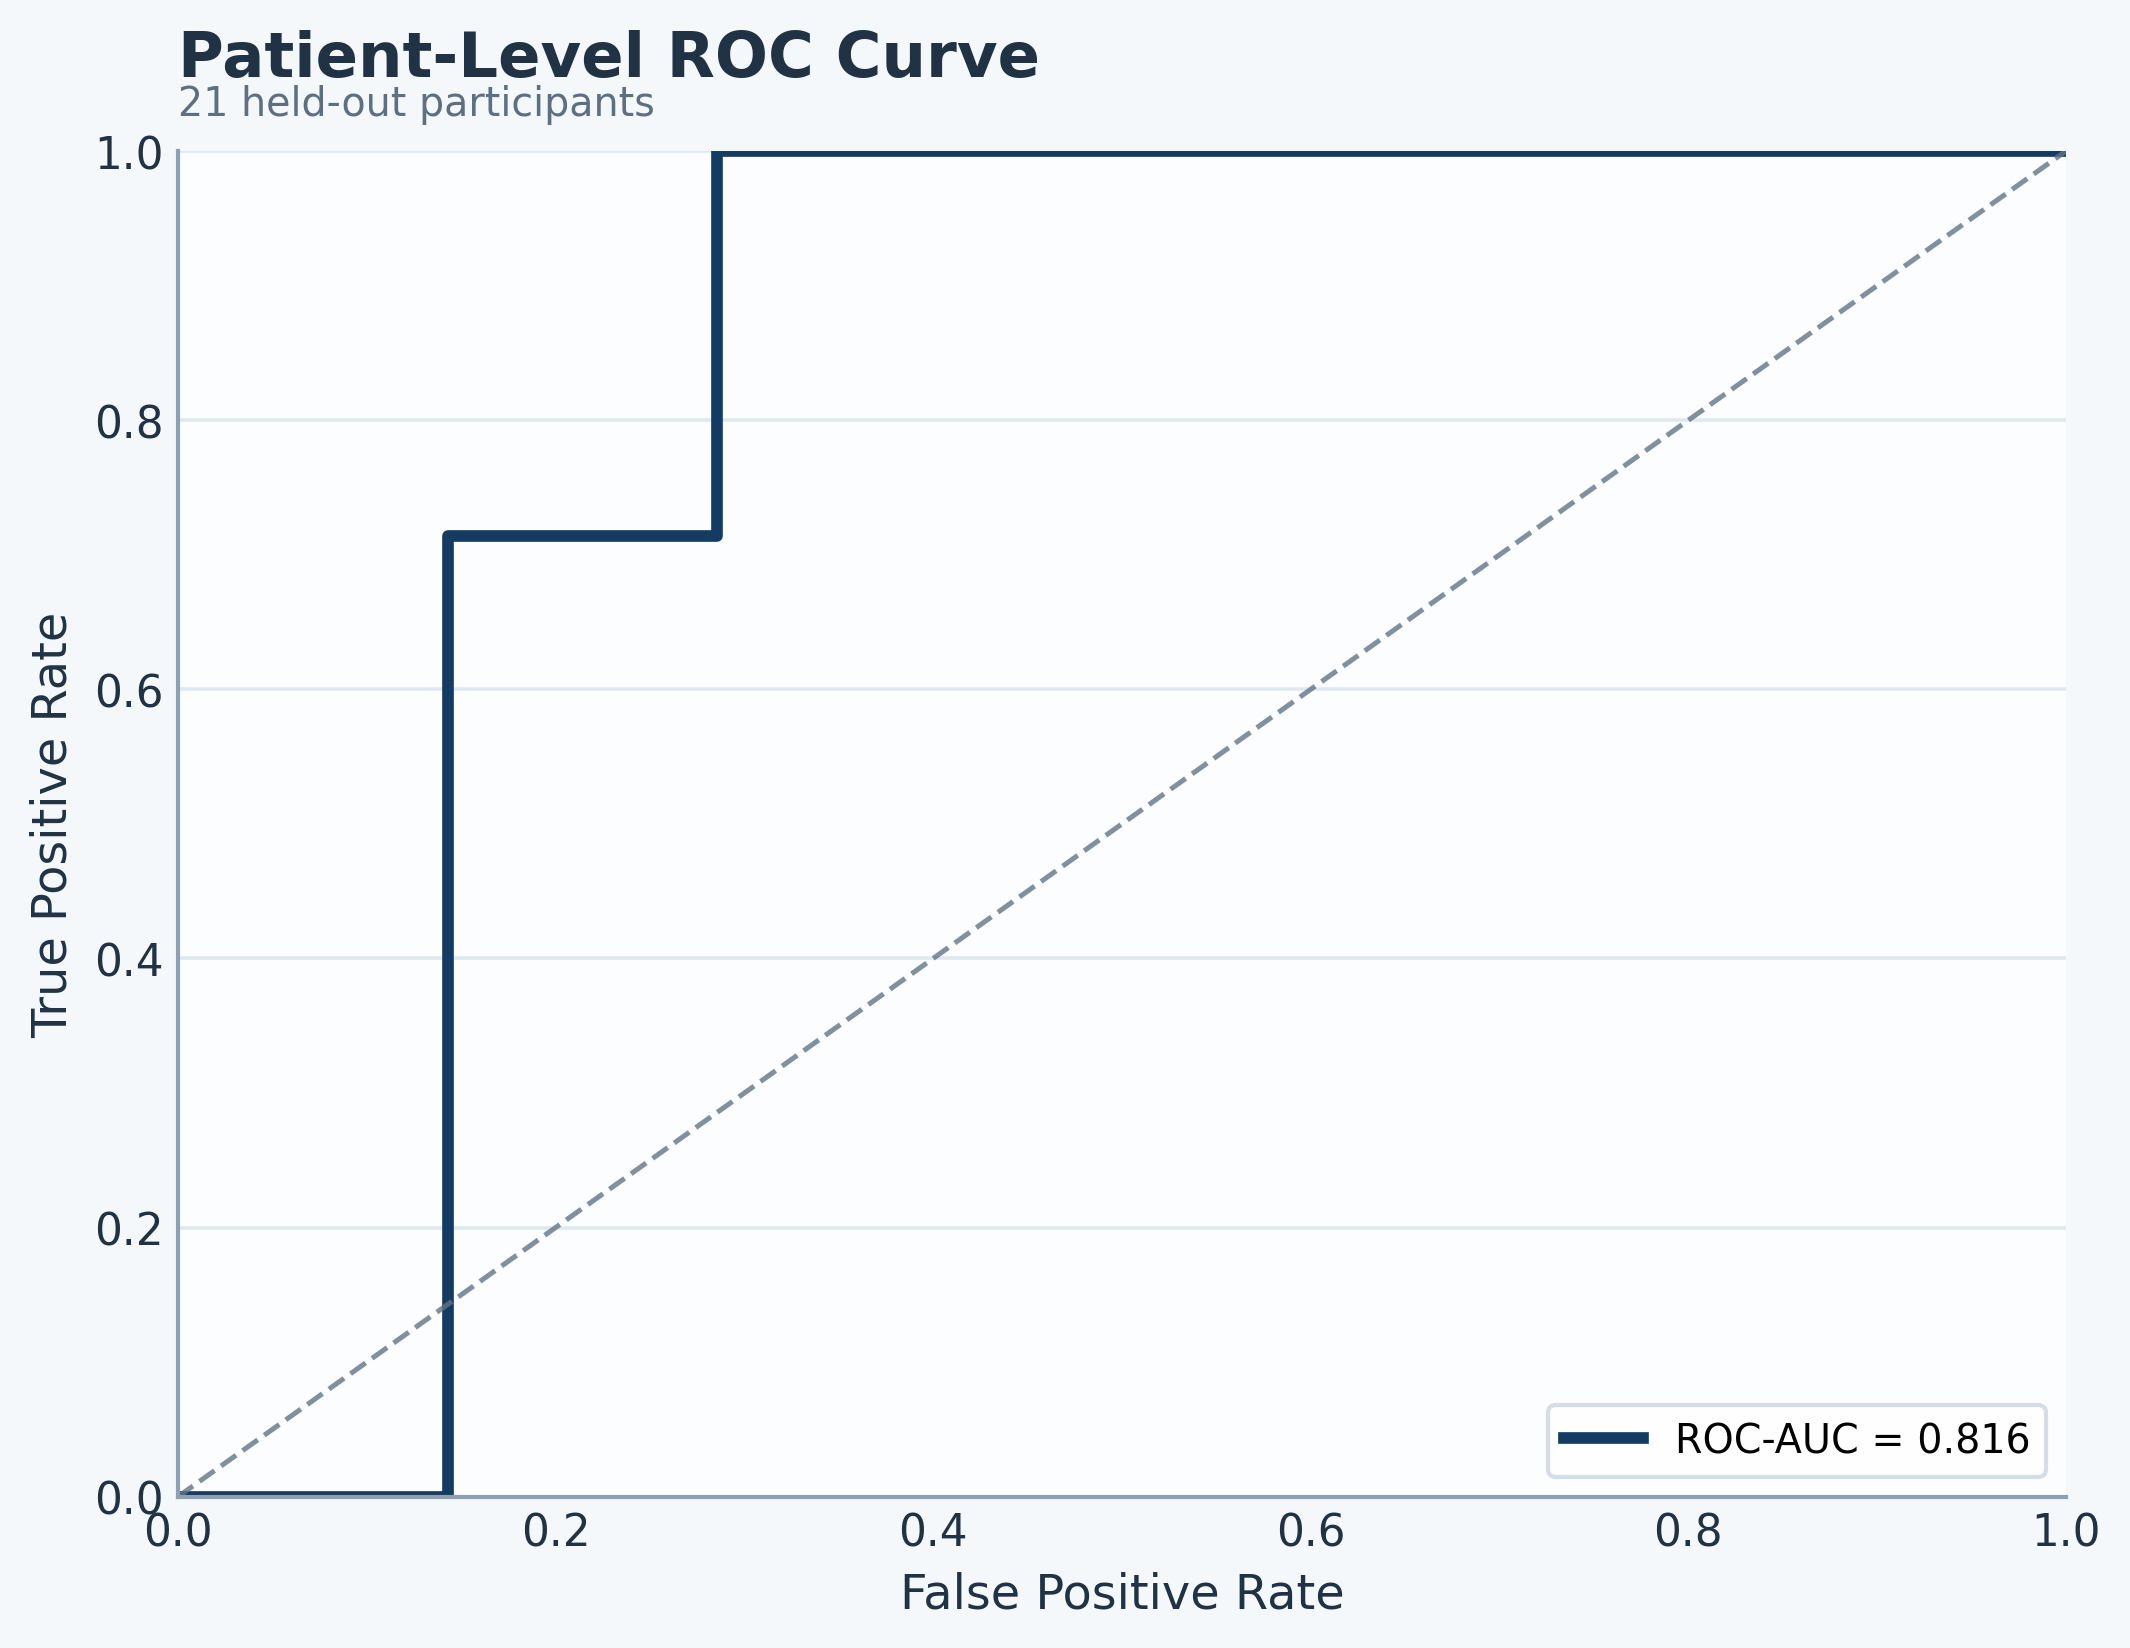
\includegraphics[width=0.94\linewidth]{main_patient_roc_curve.png}
  \caption{Patient-level ROC curve for the best hybrid run. The shaded region shows the 95\% bootstrap confidence band.}
  \label{fig:main-roc}
\end{paperinlinefigure}

The corresponding participant-level confusion counts were 12 true negatives, 5 true positives, 2 false positives, and 2 false negatives. This error profile is consistent with the balanced-accuracy summary and shows that the strongest run retained useful sensitivity without sacrificing specificity. Figure~\ref{fig:main-metrics} shows the same run in condensed metric form with 95\% bootstrap confidence intervals.

The best SVM baseline reached balanced accuracy 0.643 and ROC-AUC 0.510 [95\% CI: 0.119--0.881], with a non-significant permutation result (raw $p=0.469$, uncorrected). This weaker performance came with a much larger per-fold feature budget (\texttt{inner-k=30}) and a far larger overall candidate set. The contrast indicates that the sparse hybrid pipeline extracted stronger patient-level discrimination from a much smaller subset of features.

\begin{paperinlinefigure}
  \centering
  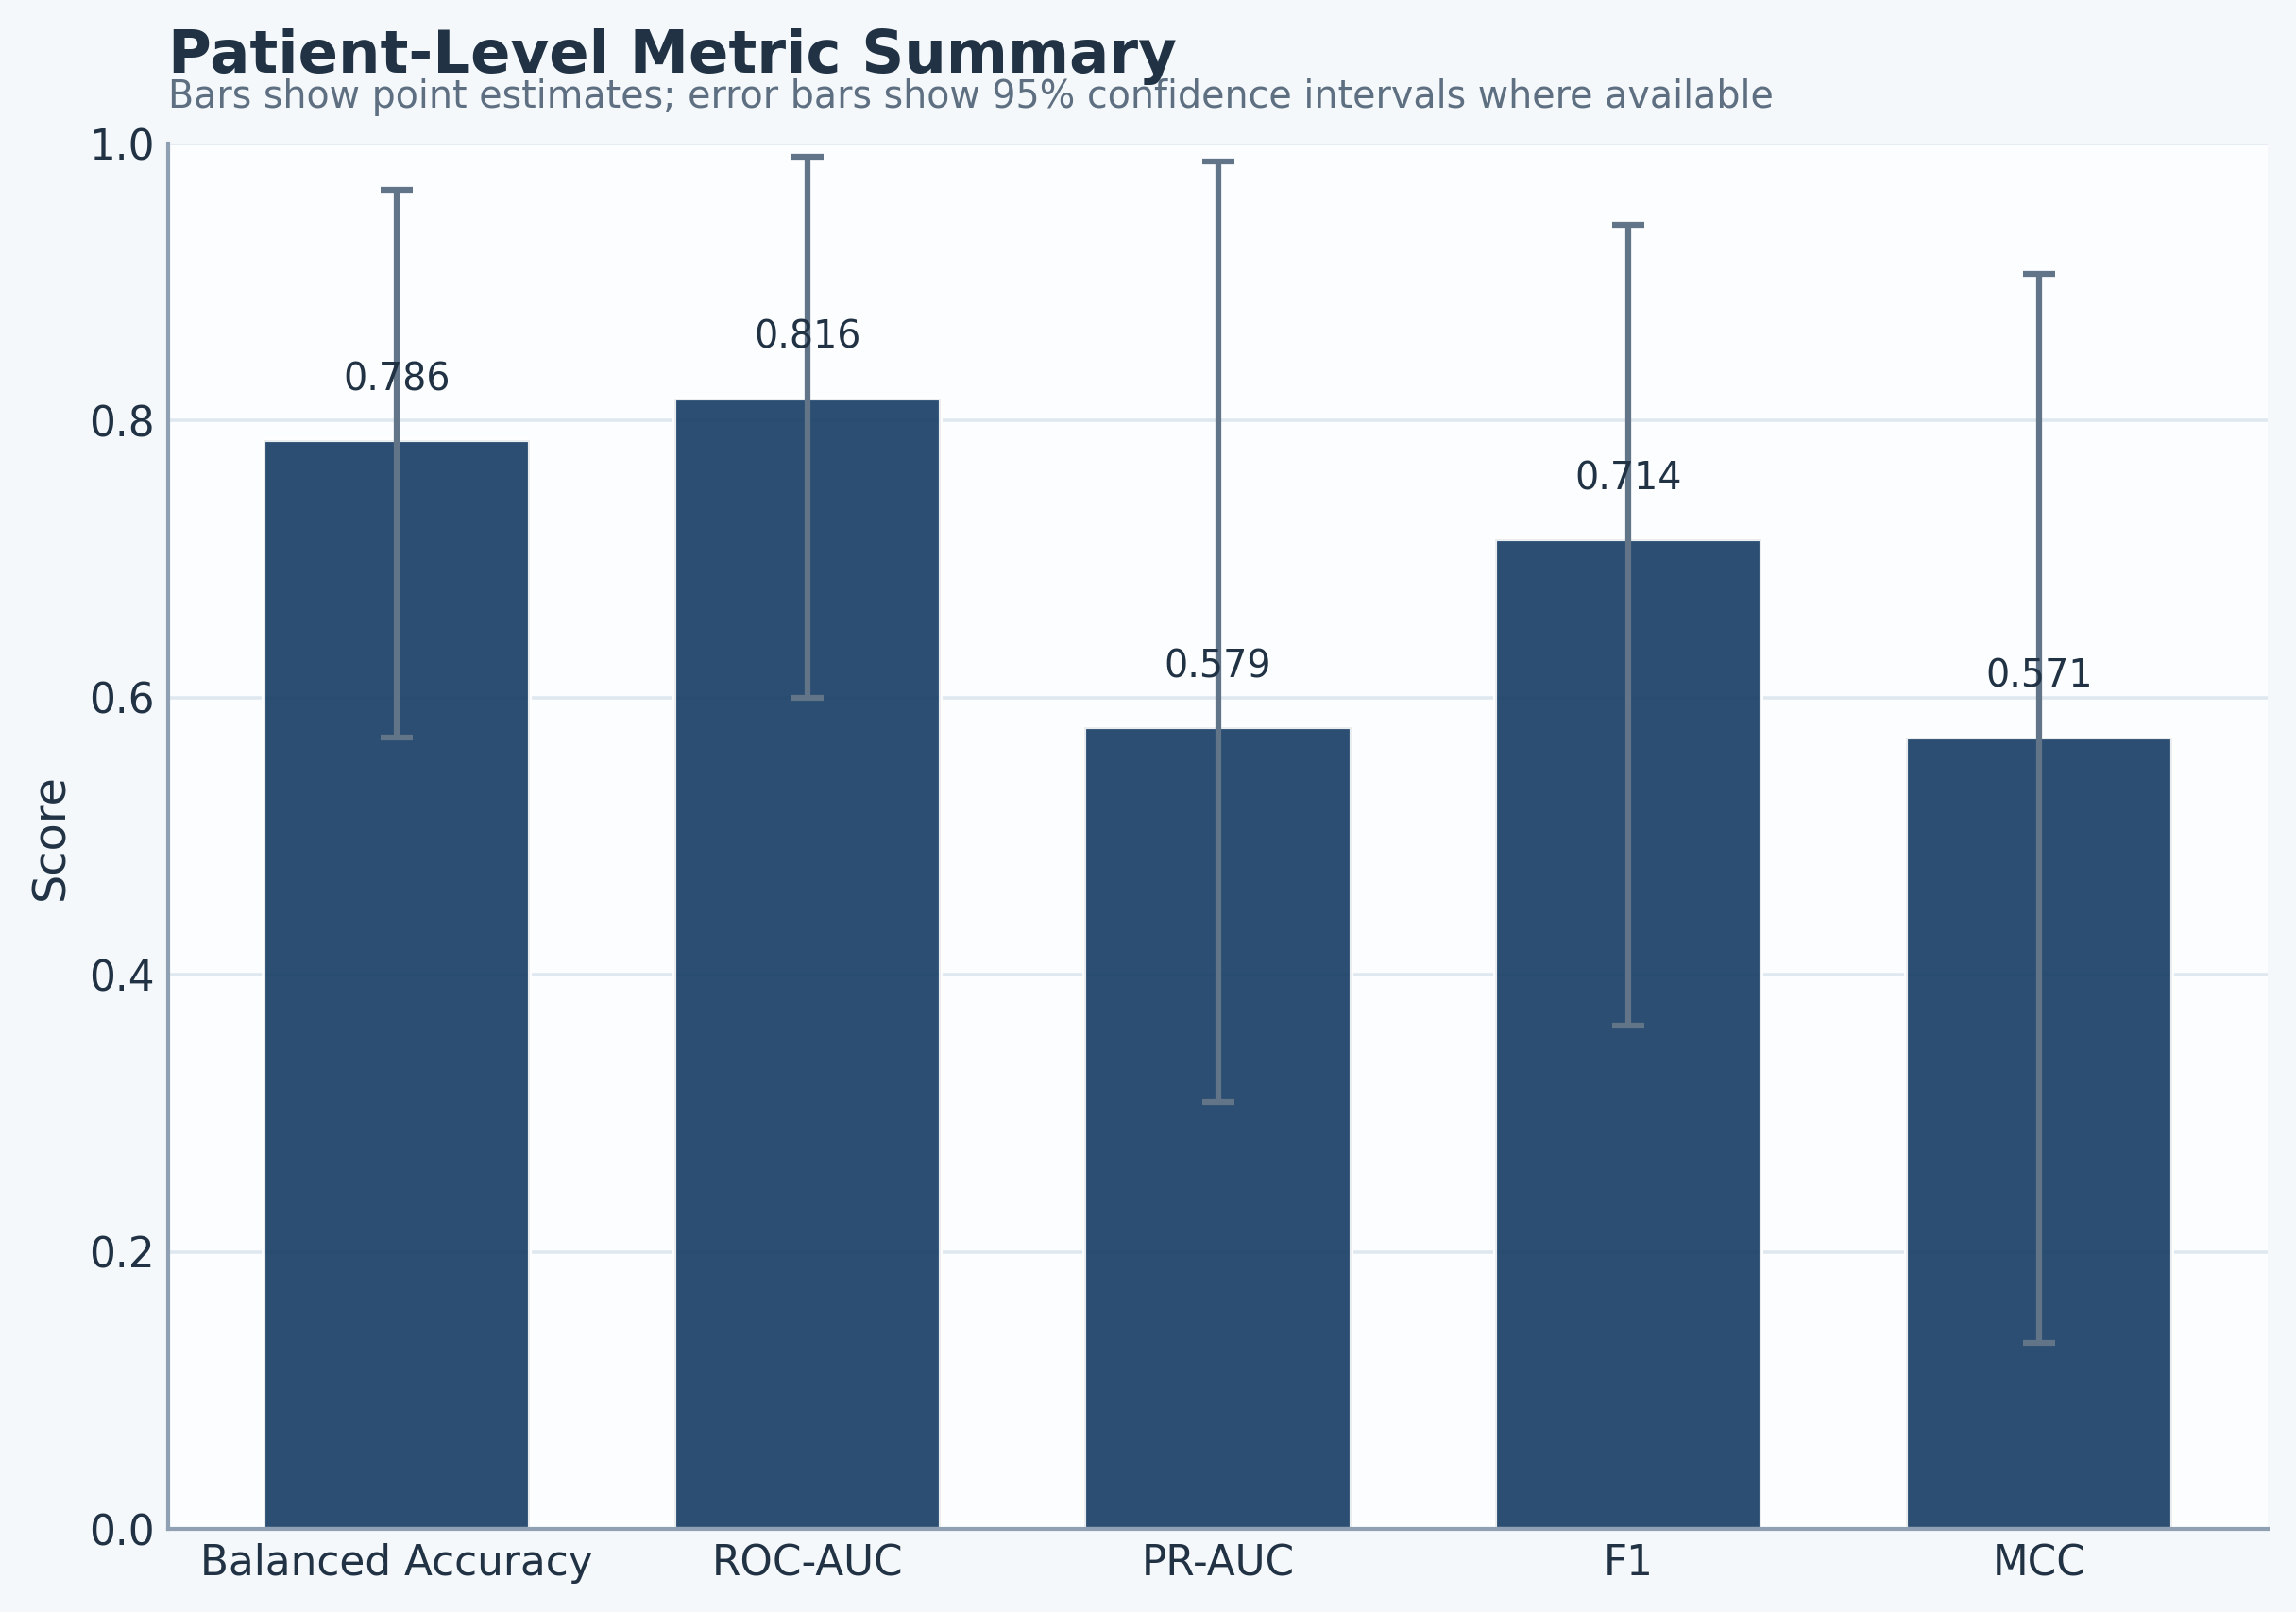
\includegraphics[width=0.94\linewidth]{main_patient_metric_summary.png}
  \caption{Patient-level metric summary for the best hybrid run. Error bars show 95\% bootstrap confidence intervals.}
  \label{fig:main-metrics}
\end{paperinlinefigure}

\begin{paperwidetable}
  \centering
  \caption{Best-performing configuration for each model family. Bootstrap confidence intervals are from 1,000 resamples at the 95\% level.}
  \label{tab:best-run-comparison}
  \resizebox{\linewidth}{!}{\begin{tabular}{lcccccccccc}
\toprule
Model & Window & Inner-k & ROC-AUC & PR-AUC & Bal.\ Acc. & F1 & MCC & Feat./fold & Unique feat. & Mean Jaccard \\
\midrule
Hybrid CNN-LSTM & 6 & 1 & 0.816 & 0.579 & 0.786 & 0.714 & 0.571 & 1.0 & 7 & 0.190 \\
Linear SVM & 8 & 30 & 0.510 & 0.411 & 0.643 & 0.533 & 0.277 & 30.0 & 103 & 0.360 \\
\bottomrule
\end{tabular}
}

  \smallskip
  \footnotesize Bootstrap 95\% CIs from 1,000 resamples. Hybrid permutation test: raw $p=0.008$; primary correction (2 model families) $p_\text{corr}=0.016$; robustness checks: max-T across 150 configurations $p_\text{corr}=0.302$, full-sweep Bonferroni $p_\text{corr}=1.00$.
\end{paperwidetable}

\subsection{Intermediate baselines and ablation at the sparsest budget}

To determine whether the hybrid architecture's advantage at \texttt{inner-k=1} reflected generic benefits of non-linearity or specific architectural properties, we evaluated eight classical classifiers and two neural baselines under the identical configuration (6 s windows, \texttt{inner-k=1}, SMOTE, LOPO equalization, same dataset and folds). All ten baselines performed at or below chance (Table~\ref{tab:intermediate-baselines}). The best classical model (Random Forest) reached ROC-AUC 0.296, compared with 0.816 for the hybrid. A 2-layer MLP (ROC-AUC 0.204) and a GAP variant of the hybrid architecture that removes self-attention and feature-pyramid fusion (ROC-AUC 0.235) both failed to exceed chance. No baseline achieved a significant permutation p-value (all $p \ge 0.9$).

An additional ablation removed SMOTE from the best hybrid configuration. Performance fell from ROC-AUC 0.816 to 0.582 (balanced accuracy 0.500, F1 0.308), indicating that SMOTE contributes substantially to the hybrid's performance in the 1-dimensional feature regime — consistent with the observation that synthetic oversampling provides the only mechanism for exposing class-boundary information when a single scalar feature is available.

These findings indicate that the hybrid CNN-LSTM's performance at extreme sparsity is not attributable to non-linearity alone, nor to SMOTE alone. The convolutional, recurrent, attention, and feature-pyramid stages, together with SMOTE-based training, appear jointly necessary to extract discriminatory signal from a single feature per fold.

\begin{paperwidetable}
  \centering
  \caption{Intermediate baseline classifiers and ablations evaluated at the best hybrid configuration (6~s, \texttt{inner-k=1}). All models used identical data, feature selection, and validation splits. Neural baselines and ablation trained on NVIDIA RTX 3090.}
  \label{tab:intermediate-baselines}
  \footnotesize
  \begin{tabular}{lcccccc}
\toprule
Model & ROC-AUC & Bal.\ Acc. & MCC & F1 & $p$ (perm.) \\
\midrule
Hybrid CNN-LSTM (best) & \textbf{0.816} & \textbf{0.786} & \textbf{0.571} & \textbf{0.714} & 0.008 \\
\midrule
Random Forest & 0.296 & 0.321 & $-$0.337 & 0.222 & 0.930 \\
Extra Trees & 0.286 & 0.500 & 0.000 & 0.375 & 0.934 \\
AdaBoost & 0.286 & 0.393 & $-$0.204 & 0.250 & 0.942 \\
Gradient Boosting & 0.276 & 0.393 & $-$0.204 & 0.250 & 0.936 \\
Decision Tree & 0.276 & 0.500 & 0.000 & 0.308 & 0.946 \\
KNN & 0.255 & 0.464 & $-$0.067 & 0.353 & 0.974 \\
SVM-RBF & 0.204 & 0.429 & $-$0.135 & 0.333 & 0.978 \\
SVM-Linear & 0.204 & 0.357 & $-$0.277 & 0.300 & 0.988 \\
\bottomrule
\end{tabular}

\smallskip
\footnotesize All models evaluated with the same configuration: window size 6~s, \texttt{inner-k}=1, SelectKBest ($F$-classif), SMOTE enabled, LOPO group equalization enabled, patient-level mean aggregation. Permutation p-values from 500 iterations. The hybrid result is shown for reference (not part of this sweep).

\end{paperwidetable}

The winning hybrid run selected an average of 1 feature per fold and yielded only 7 unique features that appeared in at least one fold across the entire participant-level validation process (Table~\ref{tab:hybrid-biomarkers}). That degree of sparsity is one of the most distinctive findings in the sweep. Hard-set overlap was modest, with a mean pairwise Jaccard value of 0.190 and a mean Kuncheva index of 0.187. Figure~\ref{fig:biomarker-frequency} shows the small candidate pool, while the overlap statistics indicate that recurrence was concentrated in a few repeatedly reappearing features rather than in a broadly shared foldwise set.

A small set of features emerged repeatedly, though not in every fold, and the selected features were dominated by temporal and frontal-temporal descriptors. The most frequently selected feature was \texttt{tp10\_spectral\_entropy}, selected in 8 of 21 folds. The next most frequent were \texttt{left\_frontal\_temporal\_diff\_gamma}, \texttt{left\_frontal\_temporal\_diff\_beta}, and \texttt{af7\_zero\_crossings}. We note that three of the seven features listed in Table~\ref{tab:hybrid-biomarkers} appear in only 1 of 21 folds; the term ``recurrent'' should be interpreted with this sparsity in mind, and the sign-consistency values for these single-fold features carry limited interpretive weight.

\begin{paperinlinefigure}
  \centering
  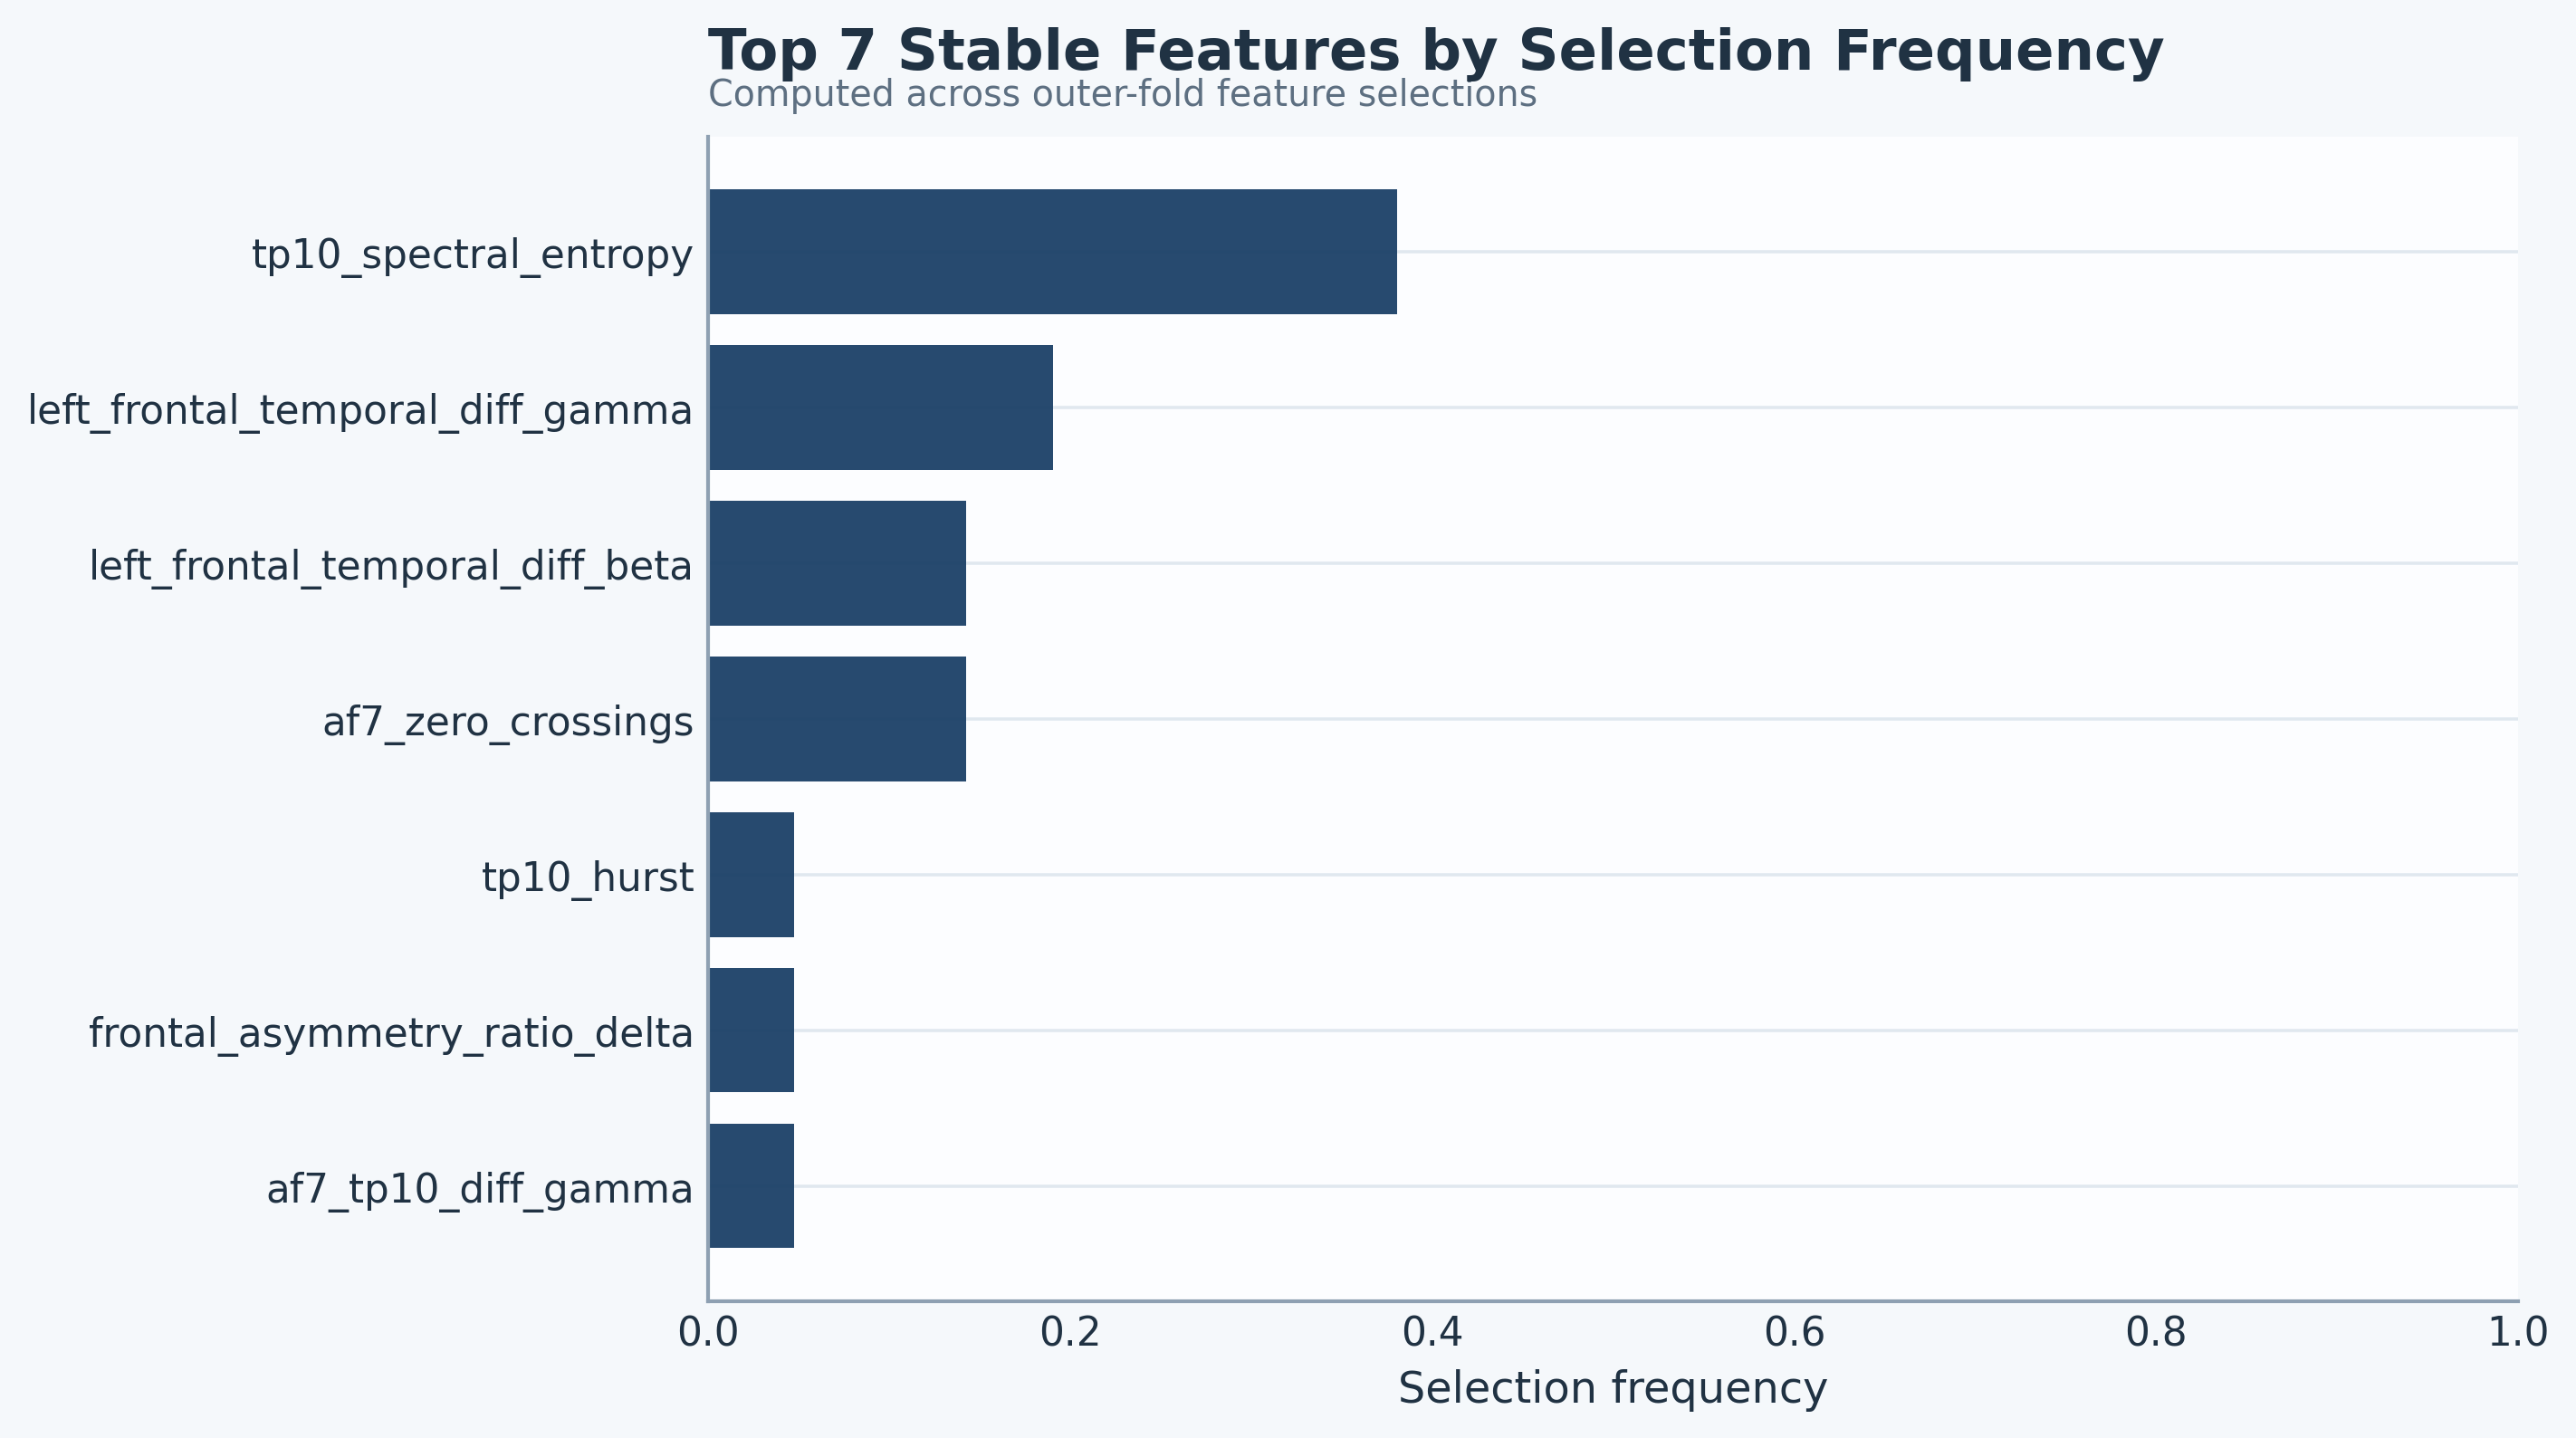
\includegraphics[width=0.94\linewidth]{biomarker_selection_frequency.png}
  \caption{Selection-frequency ranking for the features identified from the best hybrid run.}
  \label{fig:biomarker-frequency}
\end{paperinlinefigure}

\begin{paperwidetable}
  \centering
  \caption{Features from the best hybrid run that appeared in at least one fold. $\Delta$ selection is remission minus non-remission selection share. Sign consistency is 1.000 for features appearing in multiple folds; single-fold entries should be interpreted with caution.}
  \label{tab:hybrid-biomarkers}
  \resizebox{\linewidth}{!}{\begin{tabular}{lcccccc}
\toprule
Feature & Folds & Share & $\Delta$ sel. & Sign cons. & Mean $d$ & Effect direction \\
\midrule
tp10\_spectral\_entropy & 8 & 0.381 & -0.571 & 1.000 & -0.935 & Non-remission > remission \\
left\_frontal\_temporal\_diff\_gamma & 4 & 0.190 & -0.071 & 1.000 & -1.059 & Non-remission > remission \\
left\_frontal\_temporal\_diff\_beta & 3 & 0.143 & 0.000 & 1.000 & -0.915 & Non-remission > remission \\
af7\_zero\_crossings & 3 & 0.143 & 0.429 & 1.000 & 0.814 & Remission > non-remission \\
tp10\_hurst & 1 & 0.048 & 0.143 & 1.000 & -1.010 & Non-remission > remission \\
af7\_tp10\_diff\_gamma & 1 & 0.048 & 0.143 & 1.000 & -1.203 & Non-remission > remission \\
frontal\_asymmetry\_ratio\_delta & 1 & 0.048 & -0.071 & 1.000 & 0.794 & Remission > non-remission \\
\bottomrule
\end{tabular}
}
\end{paperwidetable}

\subsection{Effect-direction consistency and class-conditional patterns}

The recurrent hybrid biomarkers showed perfect mean sign consistency, with all recurrent features retaining the same effect direction across the folds in which they were selected. \texttt{tp10\_spectral\_entropy} and the frontal-temporal gamma and beta difference terms were repeatedly associated with the non-remission group, whereas \texttt{af7\_zero\_crossings} was more frequently selected in remission folds. The class-conditional selection frequencies make that separation visible at the level of foldwise recurrence (Figure~\ref{fig:biomarker-class-conditional}).

\begin{paperinlinefigure}
  \centering
  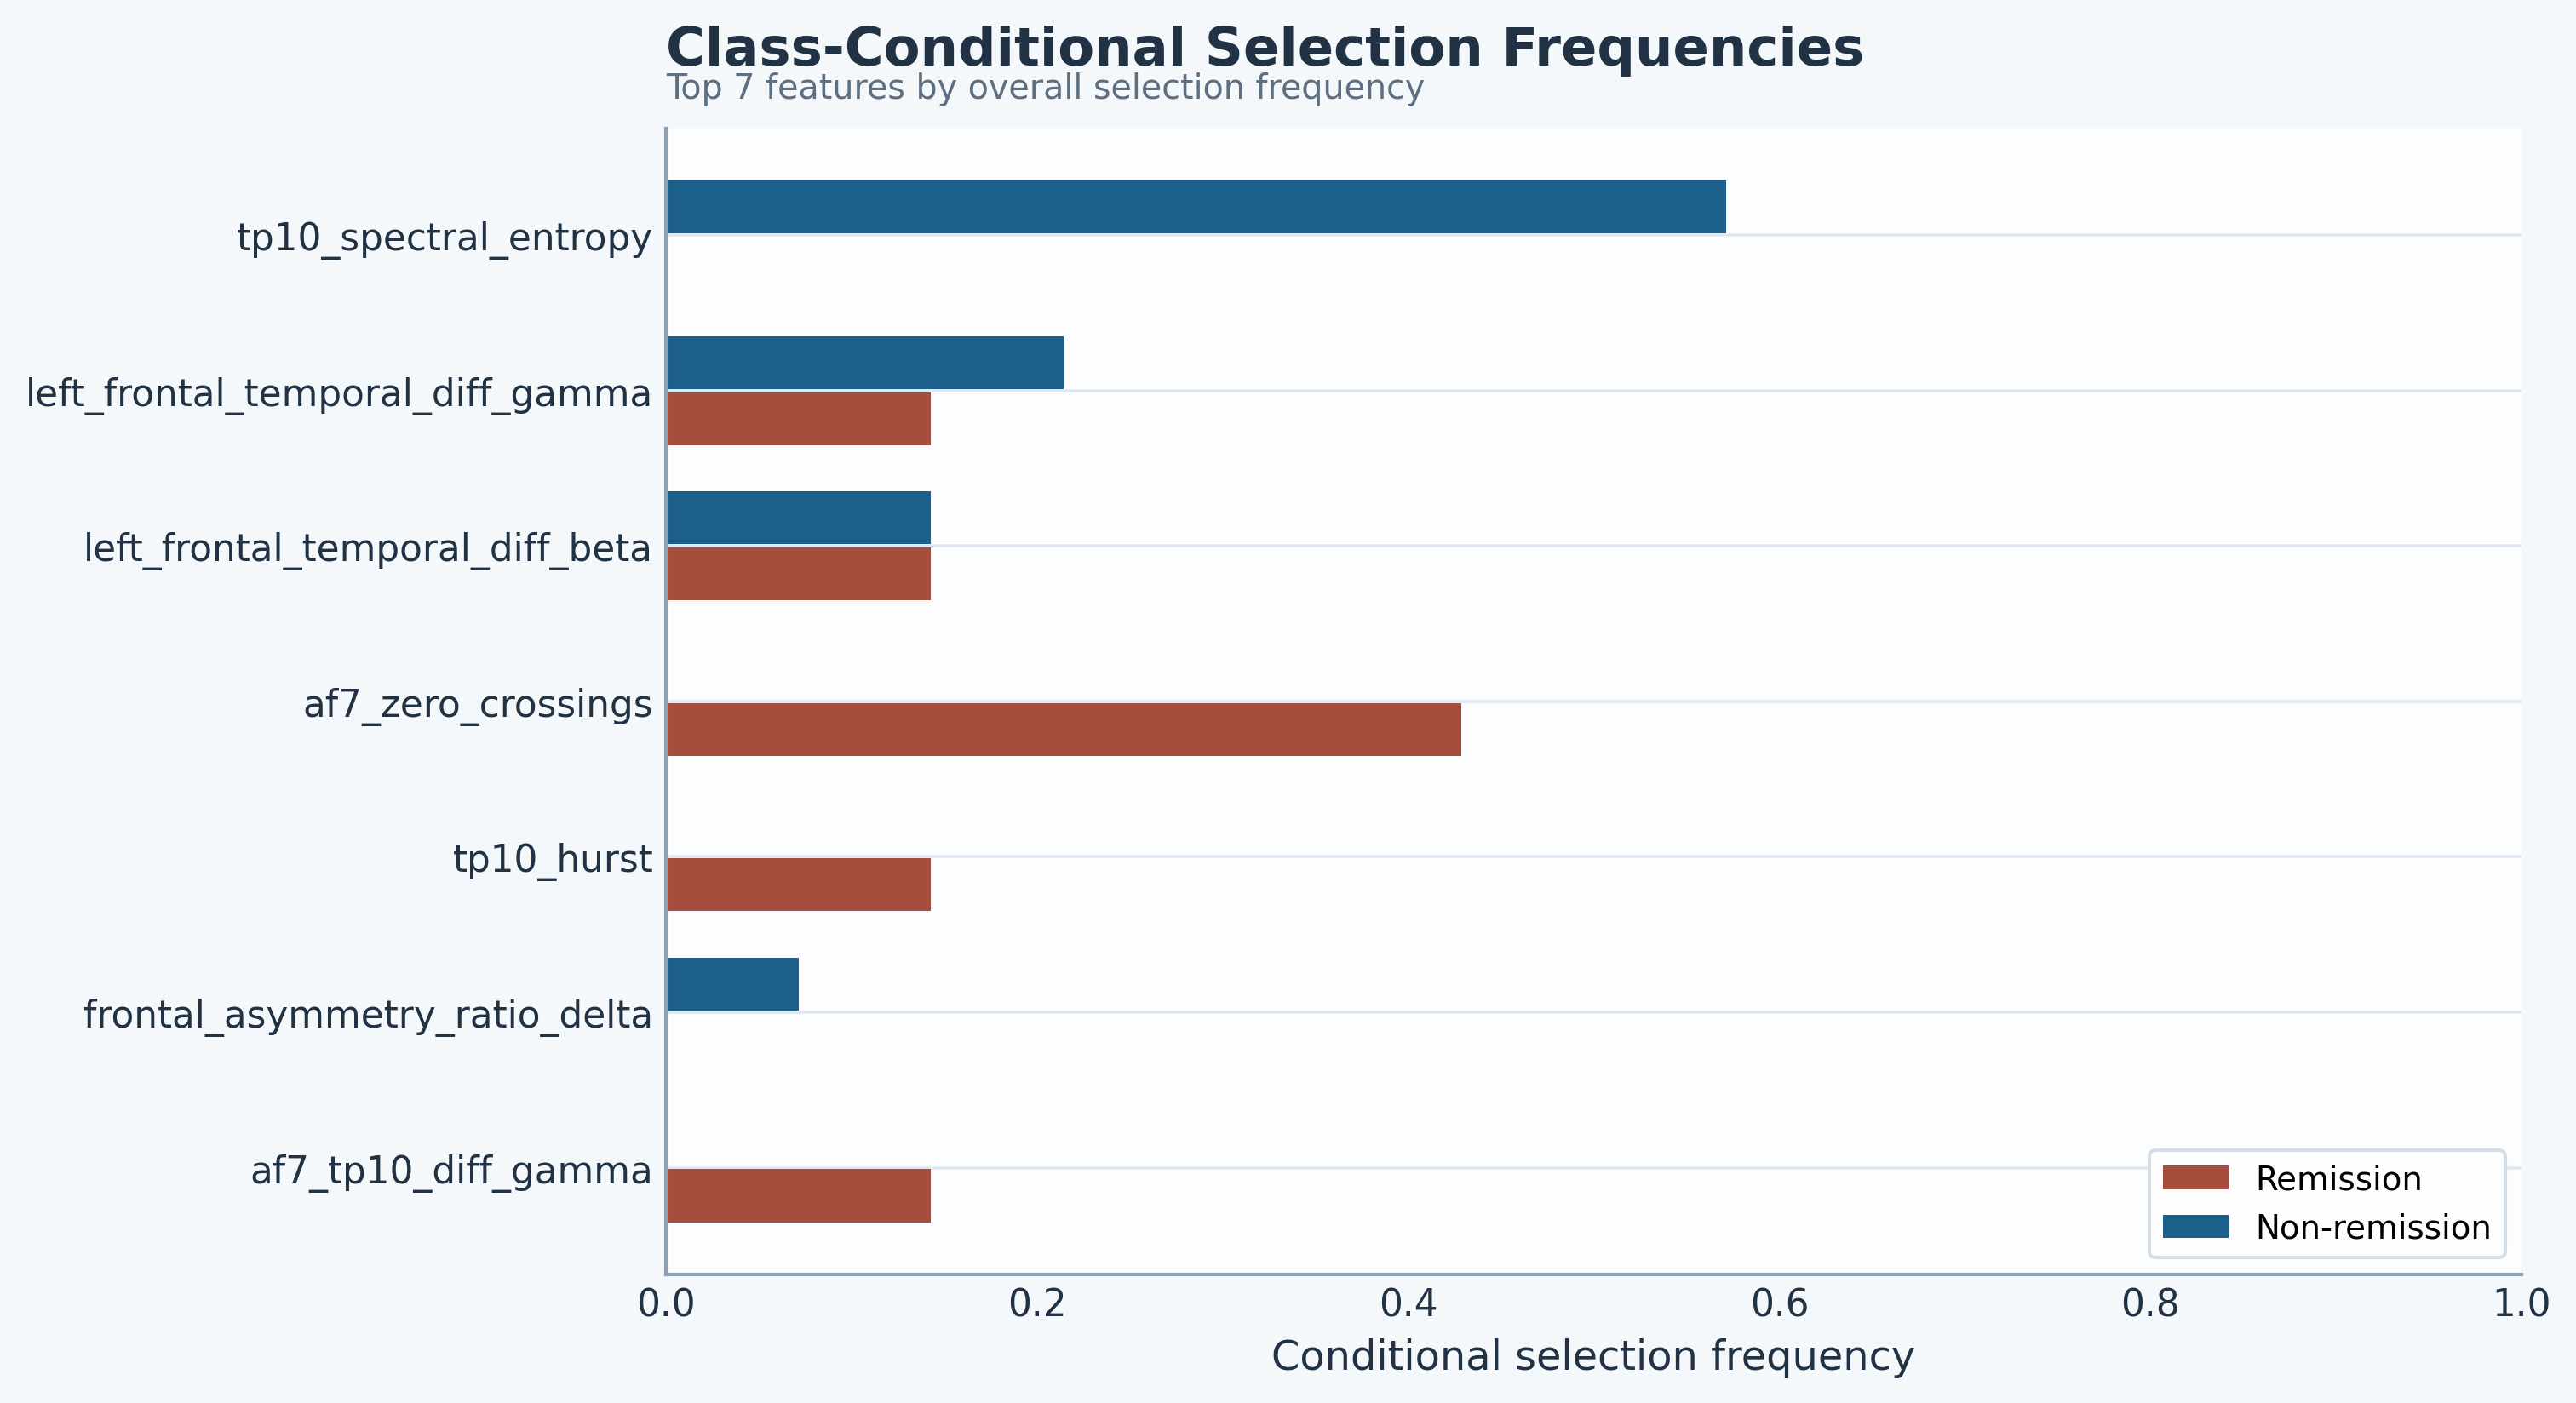
\includegraphics[width=0.94\linewidth]{figure6_class_conditional_selection.png}
  \caption{Class-conditional selection frequencies for the recurrent biomarkers from the best hybrid run. Remission is shown in red and non-remission in blue.}
  \label{fig:biomarker-class-conditional}
\end{paperinlinefigure}

The effect-size summaries followed the same broad pattern, with \texttt{af7\_zero\_crossings} retaining a positive mean effect size and the main TP10 and frontal-temporal features retaining negative mean effects (Figure~\ref{fig:biomarker-effect-size}). This distinction matters clinically. The selection-frequency deltas do not justify definitive mechanistic claims. They provide a concrete interpretation target for follow-up validation. Taken together, these results indicate that useful patient-level discrimination can be achieved with an extremely sparse feature budget, while the recurrent biomarkers retain interpretable directionality even when fold-to-fold set overlap remains modest.

\subsection{Aggregation robustness}

Patient-level metrics in the main analysis were derived by averaging window probabilities within each participant. To assess sensitivity to outlier windows, we recomputed the best hybrid run's patient-level metrics using median aggregation and 25\% trimmed-mean aggregation. Median aggregation yielded ROC-AUC 0.857, PR-AUC 0.620, and MCC 0.571; trimmed-mean aggregation yielded ROC-AUC 0.837 and MCC 0.571. Both alternative aggregation methods matched or exceeded the original mean-aggregated performance (ROC-AUC 0.816), confirming that the main results are not driven by outlier windows and that the reported mean-based metrics are conservative rather than inflated.

\begin{paperinlinefigure}
  \centering
  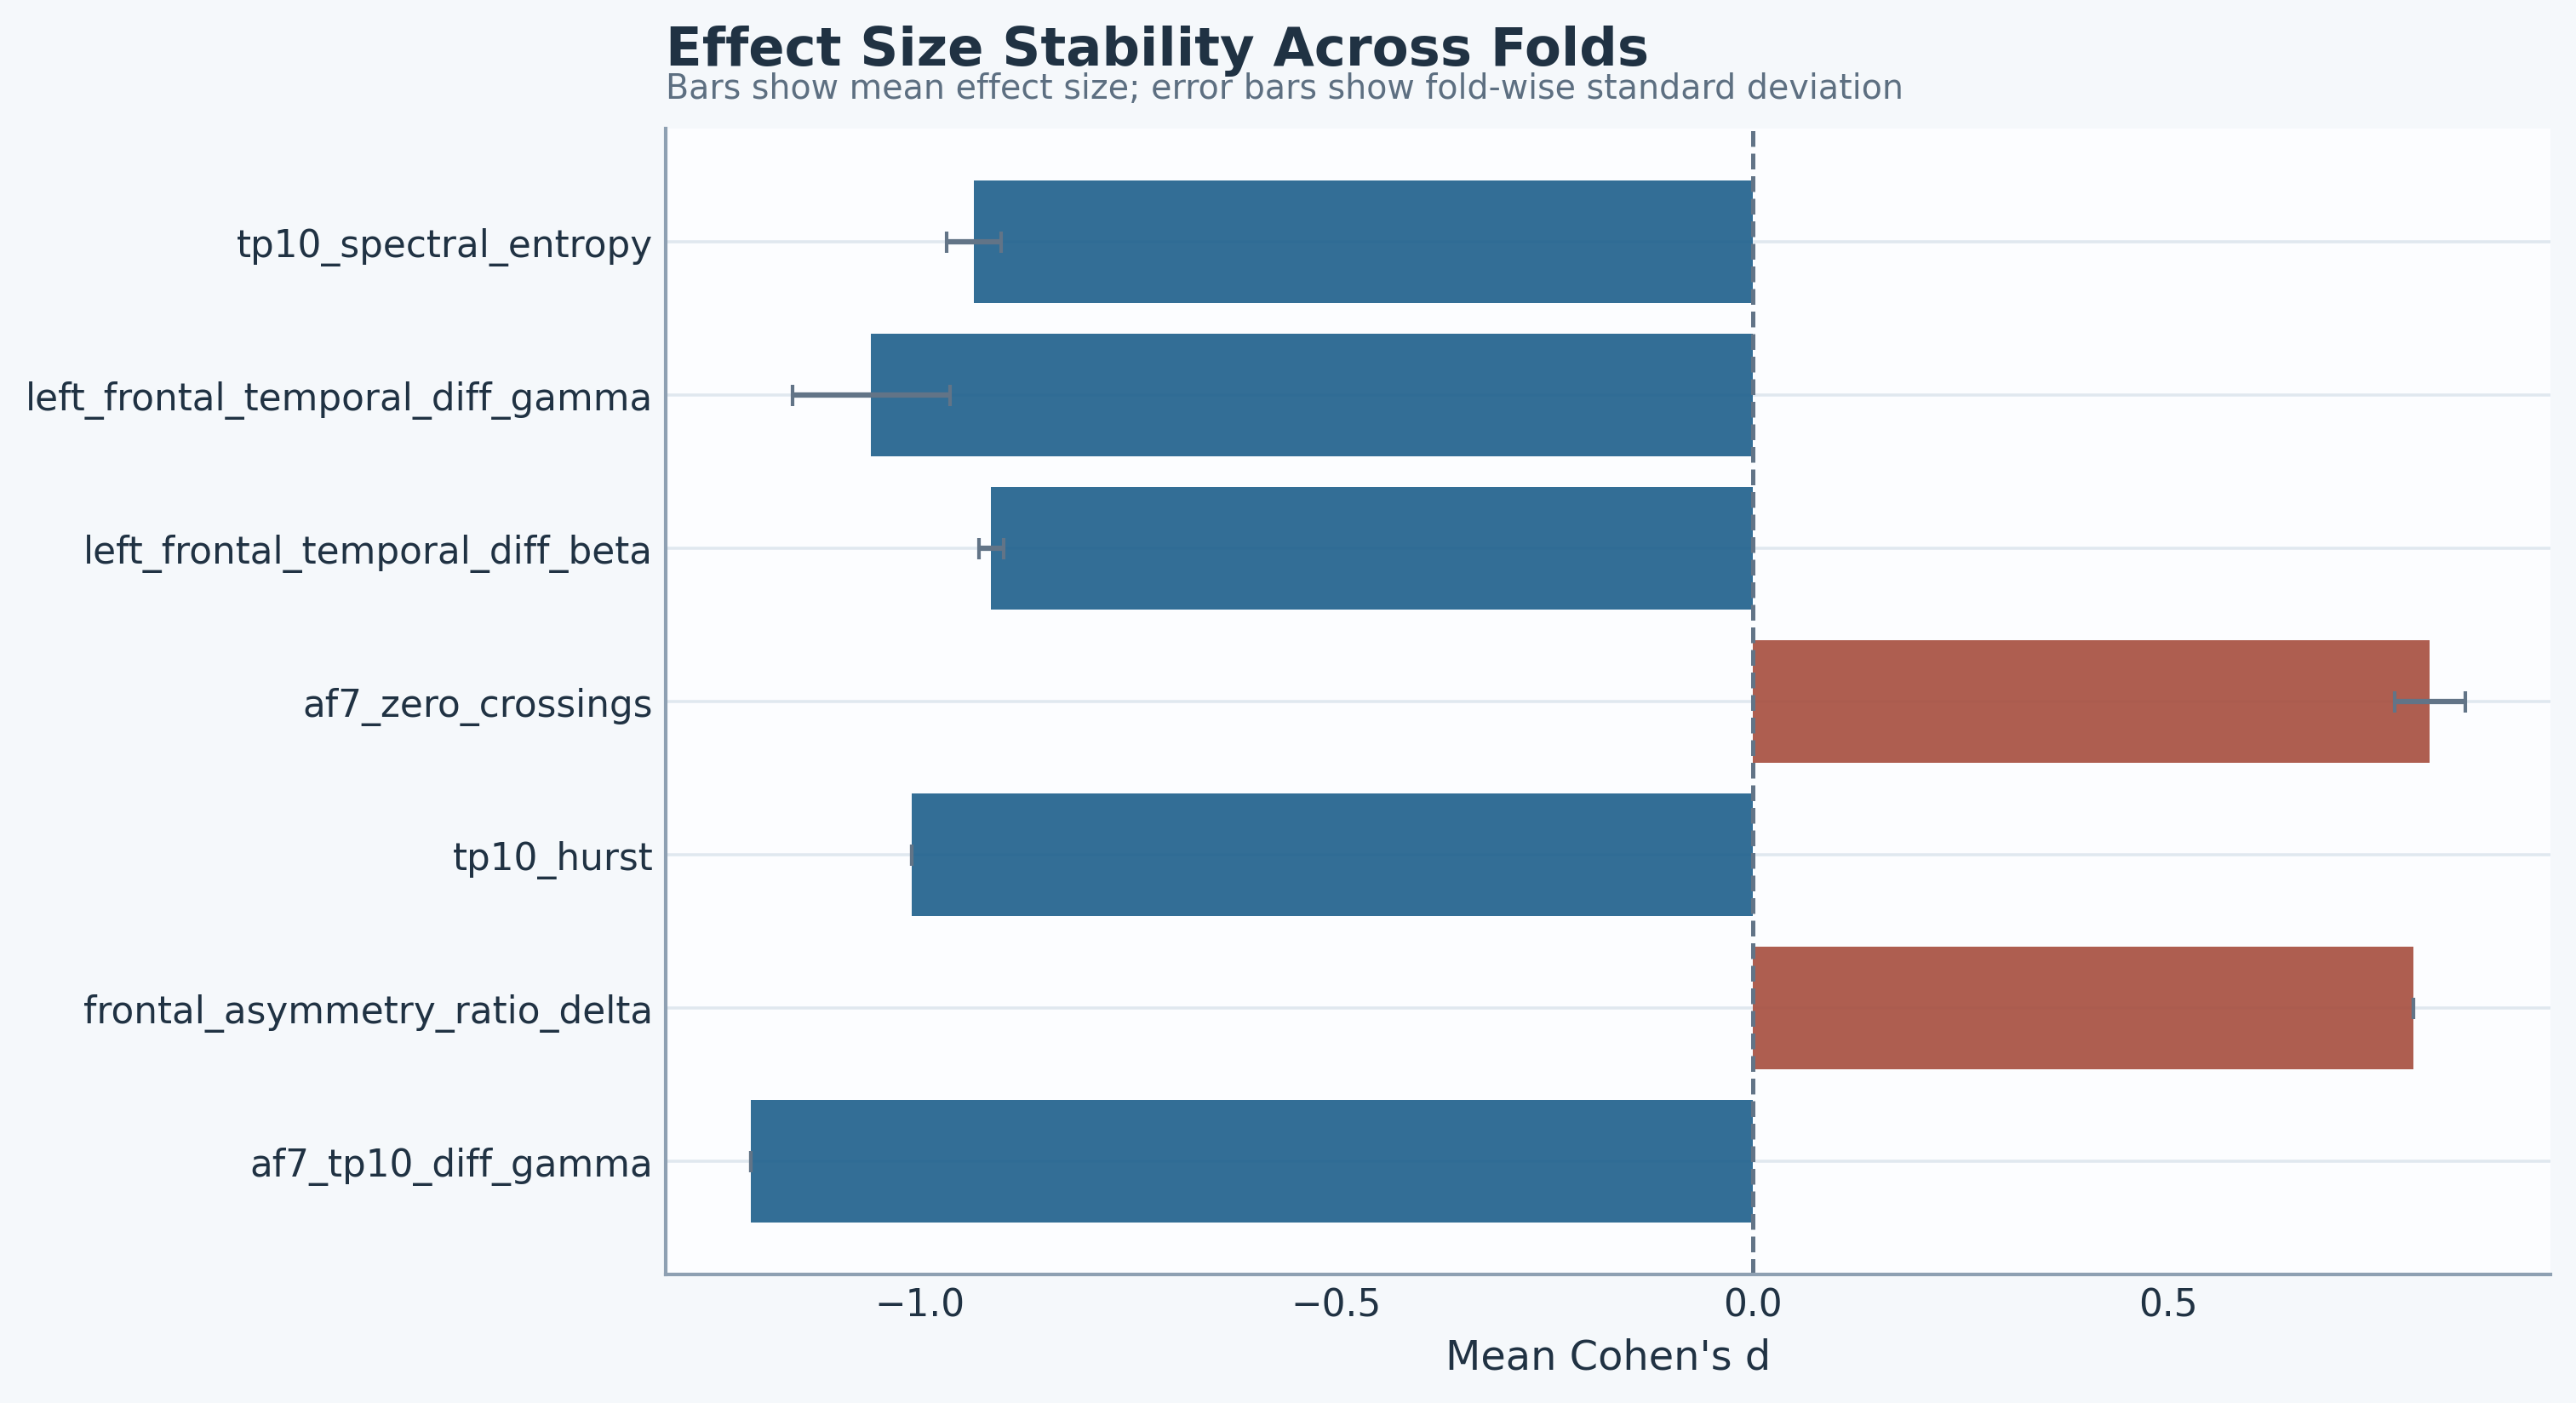
\includegraphics[width=0.94\linewidth]{figure7_effect_size.png}
  \caption{Effect-size stability for the recurrent biomarkers from the best hybrid run. Positive values indicate remission-skewed effects and negative values indicate non-remission-skewed effects.}
  \label{fig:biomarker-effect-size}
\end{paperinlinefigure}


\section*{Discussion}
The strongest patient-level discrimination in this sweep emerged from the sparsest tested configuration. The best hybrid run used \texttt{inner-k=1}, selected only 7 unique features appearing in at least one fold, and exceeded the best linear baseline by a large margin on ROC-AUC and MCC. Figure~\ref{fig:sweep-innerk-roc} also shows that this was not a generic effect of smaller feature budgets across both models. In the low-budget region, the hybrid model retained stronger ROC-AUC than the linear SVM and reached its peak performance at the sparsest tested setting, whereas the linear model reached its best ROC-AUC only after a broader per-fold budget. In this cohort, the value of the more expressive model and the value of strong sparsity appear to have operated together.

Statistical inference was assessed with permutation tests and three tiers of multiple-comparisons correction to account for the structured sweep design. The raw permutation p-value of $p=0.008$ survives the primary structured correction (2 model families, $p_\text{corr}=0.016$) at $\alpha=0.05$. As robustness checks, we computed a max-T permutation correction across all 150 configurations ($p_\text{corr}=0.302$) and a full-sweep Bonferroni ($p_\text{corr}=1.00$), the latter being mechanically uninformative given the 150-test multiplier. We adopt the 2-family correction as the primary inference because the inner-k and window-size factors represent exploratory levels of a single hypothesis rather than independent comparisons, and report all tiers for complete transparency. Several additional caveats qualify the results. The study is limited to $n=21$ participants with a 7:14 class imbalance, producing wide bootstrap confidence intervals (e.g., ROC-AUC 95\% CI: 0.600--0.990) that span both chance-level and near-perfect performance. The hybrid model's hyperparameters were inherited from a standard configuration rather than tuned specifically on this cohort; while this reduces researcher degrees of freedom, the configuration may not be optimal for the present data.

One plausible explanation for the performance gap between models is that aggressive per-fold pruning removed weak or redundant handcrafted features and exposed a compact signal set whose interactions were more useful to the hybrid architecture than to a linear decision boundary. Supporting this interpretation, eight classical classifiers and two neural baselines (2-layer MLP, GAP architecture variant) were evaluated at the identical \texttt{inner-k=1} configuration; all performed at or below chance (ROC-AUC 0.204--0.296, Table~\ref{tab:intermediate-baselines}). An additional ablation removed SMOTE from the hybrid, reducing ROC-AUC from 0.816 to 0.582. Together these results show that the full CNN-BiLSTM-attention pipeline with SMOTE-based training is jointly required — neither non-linearity alone, nor SMOTE alone, nor a simplified deep architecture suffices. With only a few retained descriptors, the convolutional, recurrent, and attention stages appear better positioned to combine complementary temporal and frontal-temporal information without dilution from a larger pool of unstable candidates. We did not compute formal paired statistical tests (e.g., DeLong or bootstrapped AUC comparison) between the two model families because the best configurations operate at different inner-k values (1 vs.\ 30). At matched inner-k values near the hybrid's optimum, the SVM operates near chance (ROC-AUC $\approx$ 0.4--0.5; Figure~\ref{fig:sweep-innerk-roc}), so the performance gap is large enough that formal testing at the matched optimum would add limited insight. The intermediate-baseline experiment (Table~\ref{tab:intermediate-baselines}) provides complementary evidence: ten alternative models all fail at inner-k=1, supporting the conclusion that the hybrid's advantage is not a statistical artifact of the sweep. This interpretation remains provisional, but it is consistent with the sweep pattern and with the marked separation between the best sparse hybrid run and the broader-budget linear baseline.

This result fits part of the EEG depression literature and supports a measured interpretation. Prior work has argued that EEG can provide clinically useful baseline markers in major depressive disorder and treatment-response settings \citep{olbrich2013_eeg,olbrich2015_personalized,leuchter2010_biomarkers}. Related discussions have also emphasized tighter biomarker discipline, better standardization, and more realistic expectations about generalization \citep{Fu2019,simmatis2023_technical,Moncy2025BD}. Machine learning studies have likewise reported encouraging treatment-response signals, including combinations of EEG and clinical covariates \citep{AlKaysi2017,jaworska2019_leveraging,oakley2022_eeg}. Other modelling studies reach similar conclusions while still exposing limits from data heterogeneity, cohort size, or insufficient interpretability \citep{shalbaf2018_nonlinear,ebrahimzadeh2021_predicting,zhdanov_svm_prediction}. Recent predictive overviews and reviews continue to highlight the same translational tension \citep{watts2022predicting,cohen2023electroencephalography}. Table~\ref{tab:sota-comparison} places the present results in the context of comparable EEG-based treatment-response prediction studies. The achieved ROC-AUC of 0.816 is competitive with prior work using larger montages and cohorts, despite the present study's substantially reduced channel count and sparse feature budget. However, direct numerical comparison is complicated by differences in clinical populations, outcome definitions, and validation methodology; the table is provided for contextual orientation rather than formal benchmarking.

\begin{paperwidetable}
  \centering
  \caption{Comparison with selected EEG-based treatment-response prediction studies in depression.}
  \label{tab:sota-comparison}
  \footnotesize
  \begin{tabular}{lcccccl}
\toprule
Study & Method & EEG channels & $n$ & AUC & Ext.\ val. & Task \\
\midrule
\citet{Moncy2024} & Deep learning (PSD features) & 4 (AF7,AF8,TP9,TP10) & 21 & 0.76$^\dagger$ & No & tDCS remission prediction \\
\citet{Xiao2025PMIP} & PLV connectivity + ML & 4 (AF7,AF8,TP9,TP10) & 21 & 0.72$^\dagger$ & No & tDCS remission prediction \\
\citet{AlKaysi2017} & SVM, RF, LR (clinical + EEG) & 19 & 80 & 0.82 & No & Antidepressant response \\
\citet{jaworska2019_leveraging} & SVM, LR (EEG + clinical) & 32 & 73 & 0.83 & No & Antidepressant response \\
\citet{oakley2022_eeg} & LORETA + SVM & 72 & 65 & 0.75 & No & Sertraline/placebo response \\
\citet{ebrahimzadeh2021_predicting} & Nonlinear EEG + classifier & 19 & 30 & 0.90 & No & Antidepressant response \\
\citet{shalbaf2018_nonlinear} & Nonlinear features + SVM & 19 & 45 & 0.88 & No & rTMS response \\
\citet{zhdanov_svm_prediction} & SVM with spectral features & 19 & 44 & 0.76 & No & Treatment response \\
\textbf{This study} & \textbf{Sparse CNN-LSTM + handcrafted features} & \textbf{4 (AF7,AF8,TP9,TP10)} & \textbf{21} & \textbf{0.82} & \textbf{No} & \textbf{tDCS remission prediction} \\
\bottomrule
\end{tabular}

\smallskip
\footnotesize $^\dagger$Estimated from reported metrics. AUC = area under the ROC curve (patient-level where available). Ext.\ val. = external validation cohort. Studies selected for relevance to EEG-based treatment response prediction in depression; the list is illustrative rather than exhaustive.

\end{paperwidetable}

The present sweep adds a feature-selection view in which larger feature budgets yield more overlap and many more unique selected features. Those larger budgets do not improve discrimination. The panels support a small set of frequently selected features with consistent direction of class separation. That reading keeps the modest Jaccard and Kuncheva scores in view and gives appropriate weight to the stronger effect-direction signal. However, the low Jaccard (0.190) and Kuncheva (0.187) scores indicate that the selected feature changes in most folds, which is a limitation for biomarker reproducibility claims. Three of the seven features appear in only a single fold, and the ``perfect'' sign consistency values for those entries should be interpreted cautiously. The Jaccard increase with larger inner-k is partly mechanical (selecting $k$ features from a fixed pool of 247 will produce more overlap by construction as $k$ increases), so this trend should not be over-interpreted as evidence of underlying signal stability. Methodologically, this framing matters because the depression EEG biomarker literature still contains substantial publication bias, limited out-of-sample validation, and known vulnerability to leakage from pre-cross-validation feature processing \citep{Widge2019,Shim2021}. The present pipeline addresses that problem by embedding selection and rebalancing inside participant-level leave-one-participant-out folds and then summarizing recurrence and directionality instead of reporting only a single global feature list \citep{Shen2025}.

The same clinical program has also supported other signal representations in recent PSD-based and PLV-based studies, which located informative response-related signal in low-density temporal and frontal-temporal patterns \citep{Moncy2024,Xiao2025PMIP}. In the present sweep, the most frequently selected features again concentrated in TP10-derived and frontal-temporal descriptors. That regional convergence supports the view that the low-montage recordings may contain response-relevant information across multiple feature families. However, the current study provides only within-cohort evidence; the generalizability of these features under different montage configurations, clinical populations, and treatment protocols remains untested.

The specific features selected in the present sweep are neurophysiologically plausible. Elevated temporal spectral entropy in non-remission participants suggests greater irregularity or complexity in the resting-state signal at the TP10 site, which overlies the temporoparietal junction — a region implicated in the default mode network and self-referential processing, both of which are dysregulated in depression. Higher entropy may reflect less organized or more variable neural dynamics that are less amenable to tDCS-induced modulation. The frontal-temporal beta and gamma difference features point toward inter-regional communication in higher frequency bands, which have been linked to top-down cognitive control and attentional processes mediated by fronto-temporal networks. tDCS applied over the dorsolateral prefrontal cortex (approximated by AF7/AF8) is thought to modulate excitability in these circuits, and baseline differences in frontal-temporal coupling may index a network's capacity to respond to such modulation. The AF7 zero-crossing count — a time-domain measure of signal volatility — showed the clearest remission-associated pattern and may capture a more dynamic or responsive frontal signal state that is conducive to stimulation-induced plasticity. These interpretations are necessarily speculative given the study's sample size and lack of independent replication, but they provide concrete, testable hypotheses for future mechanistic work.

Related tDCS studies in bipolar depression from the same group point in a similar low-montage direction. PSD-based modeling again highlighted AF7 and TP10 signal content, and PLV analyses emphasized frontal-temporal and temporoparietal synchronization patterns \citep{Moncy2025BD,Xiao2025JAD}. These bipolar studies address a different diagnosis and treatment protocol. They support reduced-montage feasibility and signal plausibility in adjacent affective cohorts.

This study has several limitations. First, the relatively small participant size ($n=21$) with a 7:14 class imbalance limits statistical power and generalizability; the wide bootstrap confidence intervals (e.g., ROC-AUC 95\% CI: 0.600--0.990) reflect this uncertainty. Although SMOTE and group equalization were applied within training folds, the fundamental class imbalance remains a constraint. Second, the primary corrected p-value ($p_\text{corr}=0.016$) survives the structured 2-family Bonferroni correction but does not survive the more conservative max-T correction across all 150 configurations ($p_\text{corr}=0.302$); replication in an independent cohort is needed. Third, there is no external validation cohort, so the reported performance and identified features cannot yet be assessed for generalizability to independent populations, alternative low-density montages, or different clinical settings. Fourth, important clinical variables such as medication status, illness duration, episode count, and psychiatric comorbidities were not available; these may influence both EEG features and treatment outcomes. Fifth, the 4-channel low-density montage trades spatial coverage for practical deployability. Recording only AF7, AF8, TP9, and TP10 captures frontal and temporal regions while omitting central, parietal, and occipital sites. This limits source-localization precision and precludes analysis of well-studied posterior alpha asymmetry markers. However, the reduced setup also enables a fully home-based, self-administered protocol that would be impractical with a 19- or 32-channel research montage, and the observed signal in these four channels supports the feasibility of this trade-off for remote tDCS monitoring. Whether a richer montage would yield higher predictive performance is an empirical question for future head-to-head studies. Sixth, the feature stability metrics (mean Jaccard 0.190, Kuncheva 0.187) indicate limited cross-fold consistency; however, median-based patient aggregation improved ROC-AUC to 0.857, suggesting that the feature signal is stable even when fold-to-fold feature identity varies. Seventh, when \texttt{inner-k=1}, SMOTE operates in a 1-dimensional feature space where the standard rationale for synthetic minority oversampling does not fully apply. The no-SMOTE ablation confirmed this concern: removing SMOTE reduced the hybrid's ROC-AUC from 0.816 to 0.582, so SMOTE is empirically essential at this setting despite the theoretical caveat. Eighth, the study does not benchmark against recent transformer-based or graph-neural-network EEG classifiers, which represent an active area of development. Ninth, the hybrid architecture contains approximately 1.2 million parameters and requires GPU acceleration for training; inference time and memory footprint, while modest for a research server, may constrain deployment on edge devices. Tenth, the SOTA comparison (Table~\ref{tab:sota-comparison}) is contextual rather than a formal benchmark due to differences in clinical populations, outcome definitions, and validation methodology between studies; direct method-level comparisons would require harmonized datasets and protocols.

The recurring features can be treated as plausible candidate features from this cohort that now warrant follow-up validation rather than as validated clinical biomarkers. Future work should test whether the same sparse feature set recurs under independent cohorts, alternative low-density montages, and explicit external validation \citep{Dagnino2023}. Adjacent response-prediction work in depression and neuromodulation provides useful targets for that next stage \citep{funk2008_prefrontal,bailey2023_concurrent,guo2024_restingstate}. Home-based and transport-oriented studies offer one clear direction for follow-up \citep{romeromarn2026_remotely,kratter2026_stanford,waller2026_transient}. More recent response-signature studies also provide relevant benchmarks for that next phase \citep{sheen2024_response,zeidabadi2025_prediction,reissmann2026_thetacordance}. Related protocol and review work in treatment-resistant depression can help frame that validation effort \citep{ulrich2025_alterations,pettorruso2024_overcoming}. These extensions should keep stringent patient-level evaluation and sparse interpretable feature budgets in the core study design, ideally with pre-registered analysis plans to limit researcher degrees of freedom.


\section*{Conclusion}
This study demonstrates that low-montage resting-state EEG can support patient-level prediction of remission outcomes in a home-based tDCS trial using an extremely sparse feature-selection framework. The strongest model achieved promising discrimination (ROC-AUC 0.816, MCC 0.571) while selecting only a small set of features, though the result does not survive correction for the full sweep of 150 configurations and should be considered exploratory.

Rather than relying on high-dimensional feature spaces, the results suggest that compact feature candidates centered on temporal entropy and frontal-temporal interactions may capture clinically relevant signal. These findings extend prior PSD-based analyses in the same cohort and support a convergent regional signal interpretation. However, the limited sample size ($n=21$), absence of an external validation cohort, and modest feature stability (Jaccard 0.190) indicate that these features should be treated as hypothesis-generating rather than as validated clinical biomarkers. Prospective validation in independent cohorts with pre-registered analysis plans is necessary before any clinical application can be considered.


\bibliography{../references,../references_analysis_subset}

\section*{Acknowledgements}
The authors express their gratitude to the participants who took part in the studies. This publication is based on research supported by grants from Flow Neuroscience (FL001), NIMH (R01MH134236), National Institute for Health and Care Research (NIHR) Health Technology Assessment (NIHR165425), NIHR Efficacy and Mechanisms Evaluation (NIHR167361), and Rosetrees Trust (CF2024M2116, CF20212104) to C.H.Y.F.


\section*{Author contributions}
A.D.Z. designed the analytical workflow, implemented the software pipeline, conducted the formal analysis, curated the data, prepared the figures, and drafted the manuscript. J.C.M. contributed to study conceptualization, data curation, methodology, software, formal analysis, visualization, and manuscript revision. M.S.S. contributed to conceptualization, methodology, investigation, supervision, project administration, funding acquisition, formal analysis, and manuscript revision. C.H.Y.F. contributed to conceptualization, methodology, investigation, supervision, project administration, funding acquisition, formal analysis, and manuscript revision. All authors reviewed and approved the final manuscript.


\section*{Additional information}
\textbf{Data availability:} The datasets analyzed in this study are not publicly available because they derive from a clinical cohort and contain sensitive participant information. Requests for access to de-identified derived data should be directed to the corresponding author and will be considered subject to ethical and institutional approval.

\textbf{Competing interests:} C.H.Y.F. received research grant support from Flow Neuroscience for the parent study. The remaining authors declare no competing interests.


\end{document}
